\documentclass[conference]{IEEEtran}
\IEEEoverridecommandlockouts
\usepackage{cite}
\usepackage{amsmath,amssymb,amsfonts}
\usepackage{algorithmic}
\usepackage{graphicx}
\usepackage{textcomp}
\usepackage{xcolor}
\usepackage{booktabs}
\usepackage{siunitx}
\usepackage{url}
\def\BibTeX{{\rm B\kern-.05em{\sc i\kern-.025em b}\kern-.08em
    T\kern-.1667em\lower.7ex\hbox{E}\kern-.125emX}}

\begin{document}

\title{Adaptive Authentication Using Machine Learning:\\
A Risk-Based Multi-Tier Security System}

\author{\IEEEauthorblockN{Satwik Basu (100751), Dr. Sreevani, Dr. Praveen Lalwani, Dr. Pushpinder Singh Patheja}
\IEEEauthorblockA{School of Computing Science Engineering and Artificial Intelligence,\\
VIT Bhopal University, Madhya Pradesh, India\\
satwikbasu03@gmail.com}}

\maketitle

\begin{abstract}
Traditional authentication mechanisms employ binary accept/reject paradigms that provide no proportional response to varying threat levels. This paper presents an Adaptive Authentication System that leverages a Random Forest classifier trained on seven behavioral and contextual features to generate continuous risk scores (0.0--1.0) for every login attempt. The system implements a configurable three-tier proportional-response framework---ALLOW, Multi-Factor Authentication (MFA), and BLOCK---enabling graduated enforcement based on tunable thresholds. We present this work as a reproducible proof-of-concept: the model is trained and evaluated on a synthetic benchmark of 10,000 authentication events, with an adversarial suite of 1,500 scenarios spanning 21 attack profiles across three risk categories. On this benchmark the model achieves 94.45\% accuracy (ROC-AUC 0.9019), with 5-fold cross-validation at 94.91\% $\pm$ 0.27\%. Because the adversarial suite is generated from the same rule set that produces the training labels, the near-perfect detection we observe on high-risk profiles should be read as an upper bound that likely overstates real-world performance rather than as a security guarantee. A comparative study against four baselines (XGBoost, Logistic Regression, SVM, KNN) motivates Random Forest on the grounds of interpretability and inference latency (43 ms median) rather than accuracy. A feature-ablation study confirms that removing Threat Score alone drops accuracy by 10.65 percentage points, revealing that the feature's dominance is partly an artifact of label construction; the remaining features nonetheless contribute a genuine 7.1~pp uplift. An adaptive-adversary evasion-cost analysis across 1{,}737 blocked samples shows that 100\% of attackers evade by changing on average 1.03 features, with Threat Score as the dominant lever (52.5\%)---exposing single-feature brittleness that the fixed benchmark alone obscures. We provide a reference REST deployment to demonstrate that the full pipeline operates within real-time latency constraints, and release all code, data, and evaluation scripts for reproducibility.
\end{abstract}

\begin{IEEEkeywords}
Adaptive Authentication, Risk-Based Authentication, Machine Learning, Random Forest, Multi-Factor Authentication, Cloud Security
\end{IEEEkeywords}

\section{Introduction}
Authentication is the cornerstone of digital security, yet the predominant paradigm remains fundamentally binary: a user either provides correct credentials and gains full access, or fails and is denied entirely. This static approach provides no defense against credential theft via phishing, data breaches, or brute-force attacks---scenarios where an attacker possesses valid credentials but exhibits anomalous behavioral patterns \cite{freeman2016}.

Risk-Based Authentication (RBA) addresses this limitation by incorporating contextual signals---such as geographic location, device fingerprint, and temporal patterns---to dynamically assess the risk of each login attempt \cite{wiefling2019}. Major technology companies (Google, Microsoft, Facebook) deploy proprietary RBA systems, but their implementations remain opaque, hindering academic analysis and reproducibility \cite{wiefling2021}.

The contributions of this paper are as follows:
\begin{itemize}
\item An explicit threat model for credential-theft adversaries that maps attacker capabilities to the contextual features expected to resist them.
\item A configurable three-tier proportional-response framework (ALLOW/MFA/BLOCK) with tunable dual thresholds, replacing the binary accept/reject decision with graduated enforcement.
\item A Random Forest risk-scoring engine over seven contextual features, evaluated on a synthetic benchmark with a full baseline comparison against XGBoost, Logistic Regression, SVM, and KNN.
\item A \textit{feature-ablation study} (leave-one-out and single-feature isolation) that quantifies per-feature dependence, confirms that Threat Score removal drops accuracy by 10.65~pp, and disentangles the label-circularity artifact from genuine predictive signal.
\item An \textit{adaptive-adversary evasion-cost} analysis that evaluates the decision boundary against a strategic attacker rather than a fixed rule set---measuring how much effort, and which feature levers, are needed to evade a block---and thereby exposes the model's reliance on a single spoofable feature.
\item A reference REST deployment demonstrating that the end-to-end pipeline meets a real-time latency budget, with full open-source release of code, data, and evaluation scripts.
\end{itemize}

\section{Related Work}
\subsection{Risk-Based Authentication}
Freeman et al. \cite{freeman2016} proposed a statistical framework for risk-based authentication using IP address and device features, establishing the theoretical foundation for context-aware login security. Wiefling et al. \cite{wiefling2019} conducted the first large-scale empirical study of RBA deployment at major web services. Their subsequent work \cite{wiefling2021}, \cite{unsel2023} produced open-source RBA implementations and evaluation benchmarks, hosted at riskbasedauthentication.org.

\subsection{Machine Learning in Authentication}
ML-based approaches to authentication security include anomaly detection using Isolation Forests \cite{liu2008}, behavioral biometrics via LSTM networks \cite{acien2021}, and ensemble methods for intrusion detection \cite{zhang2020}. Random Forest classifiers have demonstrated strong performance in network security applications due to their robustness to mixed feature types and inherent interpretability \cite{breiman2001}. Gradient boosting methods (XGBoost) \cite{chen2016} offer competitive accuracy but with reduced interpretability.

\subsection{Gap Analysis}
Existing work exhibits three limitations our system addresses: (1) binary risk classification without proportional response, (2) absence of end-to-end deployment documentation, and (3) lack of a reproducible adversarial evaluation with multiple attack profiles. The closest related work by Wiefling et al. \cite{unsel2023} provides an OpenStack plugin but focuses on the Freeman algorithm without ML-based risk scoring. Table \ref{tab:positioning} positions our contribution against representative prior work. We stress that our adversarial evaluation is conducted on synthetic, rule-generated data; the corresponding column therefore denotes methodological coverage, not validation on real attacks.

\begin{table}[t]
\caption{Positioning Against Representative Prior Work}
\label{tab:positioning}
\centering
\setlength{\tabcolsep}{4pt}
\begin{tabular}{@{}lcccc@{}}
\toprule
Work & ML risk & Proportional & Deploy- & Adversarial \\
 & scoring & response & ment & eval. \\
\midrule
Freeman \cite{freeman2016} & -- & -- & -- & -- \\
Wiefling \cite{wiefling2019} & -- & -- & -- & -- \\
Unsel \cite{unsel2023} & -- & -- & \checkmark & -- \\
This work & \checkmark & \checkmark & \checkmark & \checkmark$^{\dagger}$ \\
\bottomrule
\end{tabular}
\\[2pt]
\footnotesize $^{\dagger}$Synthetic benchmark only; not validated on real attack traffic.
\end{table}

\section{System Architecture}
\subsection{Dual-Mode Design}
The system operates in two modes: \textit{local mode} using SQLite and in-memory caching for development and research, and \textit{cloud mode} using AWS RDS (PostgreSQL), ElastiCache (Redis), and S3 for production deployment. Mode selection is controlled via environment variables with automatic fallback, ensuring zero code changes between environments.

\subsection{Authentication Pipeline}
The authentication flow operates as follows:
\begin{enumerate}
\item User submits credentials (username + password).
\item System extracts 7 contextual features from the request.
\item Random Forest model computes risk score $r \in [0.0, 1.0]$.
\item Three-tier decision is applied per (\ref{eq:decision}).
\item Decision, risk score, and contributing factors are logged for audit.
\end{enumerate}

\begin{equation}
\label{eq:decision}
\text{Decision}(r) =
\begin{cases}
\text{ALLOW}, & r < 0.3 \\
\text{MFA (TOTP challenge)}, & 0.3 \le r < 0.7 \\
\text{BLOCK (deny + rate-limit)}, & r \ge 0.7
\end{cases}
\end{equation}

\subsection{Database Schema}
The system uses four primary tables: \textit{User} (credentials, TOTP secrets), \textit{LoginLog} (audit trail with risk scores), \textit{Plan} (subscription tiers), and \textit{APIKey} (key management with usage tracking).

\section{Threat Model}\label{sec:threat}
We consider an adversary whose goal is to obtain authenticated access using \textit{valid} credentials acquired through phishing, credential stuffing, or breach reuse. Credential compromise itself is out of scope; we assume the attacker already holds a correct username/password pair, which is precisely the setting where binary authentication fails.

We assume the following adversary capabilities: (C1) knowledge of the victim's credentials; (C2) the ability to originate requests from arbitrary IP addresses and geographic locations, including via VPNs and proxies; (C3) the ability to spoof coarse device fingerprints such as user-agent and device type; and (C4) no knowledge of the victim's historical login timing or of the deployed model's parameters.

The contextual features are intended to raise the cost of these capabilities to differing degrees. Location and distance features (Country, Region, Distance) resist C2 by requiring the attacker to additionally co-locate with, or accurately mimic, the victim's usual geography. Threat Score (IP reputation) resists C2 when the attacker reuses flagged infrastructure but degrades against clean residential proxies. Temporal features (Hour of Day) resist C4, since the attacker lacks the victim's timing distribution. Device features offer only limited resistance under C3. The system does \textit{not} defend against an adversary who fully replicates the victim's context---same location, device, and timing---which constitutes the residual risk that richer behavioral biometrics (see Limitations) would be needed to address.

\section{Machine Learning Model}
\subsection{Feature Engineering}
Each login attempt is characterized by seven features, summarized in Table \ref{tab:features}.

\begin{table}[t]
\caption{Feature Set for Risk Assessment}
\label{tab:features}
\centering
\begin{tabular}{@{}clll@{}}
\toprule
\# & Feature & Type & Rationale \\
\midrule
1 & Country & Categorical & Geo-location anomaly \\
2 & Region & Categorical & Continental risk zone \\
3 & Hour of Day & Numerical & Temporal pattern \\
4 & Device Type & Categorical & Device fingerprint \\
5 & Prev. Login & Binary & Account history \\
6 & Threat Score & Numerical & IP reputation (0--100) \\
7 & Distance (km) & Numerical & Impossible travel \\
\bottomrule
\end{tabular}
\end{table}

\begin{table}[t]
\caption{Classification Performance Metrics}
\label{tab:perf}
\centering
\begin{tabular}{@{}lcc@{}}
\toprule
Metric & Safe Class & Risk Class \\
\midrule
Precision & 0.9428 & 0.9522 \\
Recall & 0.9892 & 0.7829 \\
F1 Score & 0.9654 & 0.8593 \\
\midrule
Overall Accuracy & \multicolumn{2}{c}{0.9445} \\
ROC-AUC & \multicolumn{2}{c}{0.9019} \\
PR-AUC & \multicolumn{2}{c}{0.8565} \\
\bottomrule
\end{tabular}
\end{table}

\subsection{Training Data Generation}
We generate 10,000 synthetic authentication events spanning 200 countries using five domain-expert risk injection rules: (1) high threat score ($>$ 70), (2) long distance ($>$ 3000 km), (3) unusual hours (0:00--5:00), (4) combined risk factors, and (5) high-risk country origin. A 5\% label noise injection ensures model robustness to imperfect ground truth---a standard practice when real authentication logs are unavailable due to privacy regulations (GDPR, CCPA) \cite{freeman2016}, \cite{wiefling2019}.

\subsection{Model Configuration}
We employ a Random Forest classifier with 200 estimators, maximum depth of 18, minimum samples split of 5, and minimum samples leaf of 2. The 80/20 train-test split uses stratified sampling to preserve class distribution ($\sim$21.6\% positive rate).

\section{Evaluation}
\subsection{ML Performance Metrics}
Table \ref{tab:perf} reports per-class and overall classification performance, and Fig. \ref{fig:roc} and Fig. \ref{fig:cm} present the ROC curve and confusion matrices.

\begin{figure}[t]
\centering
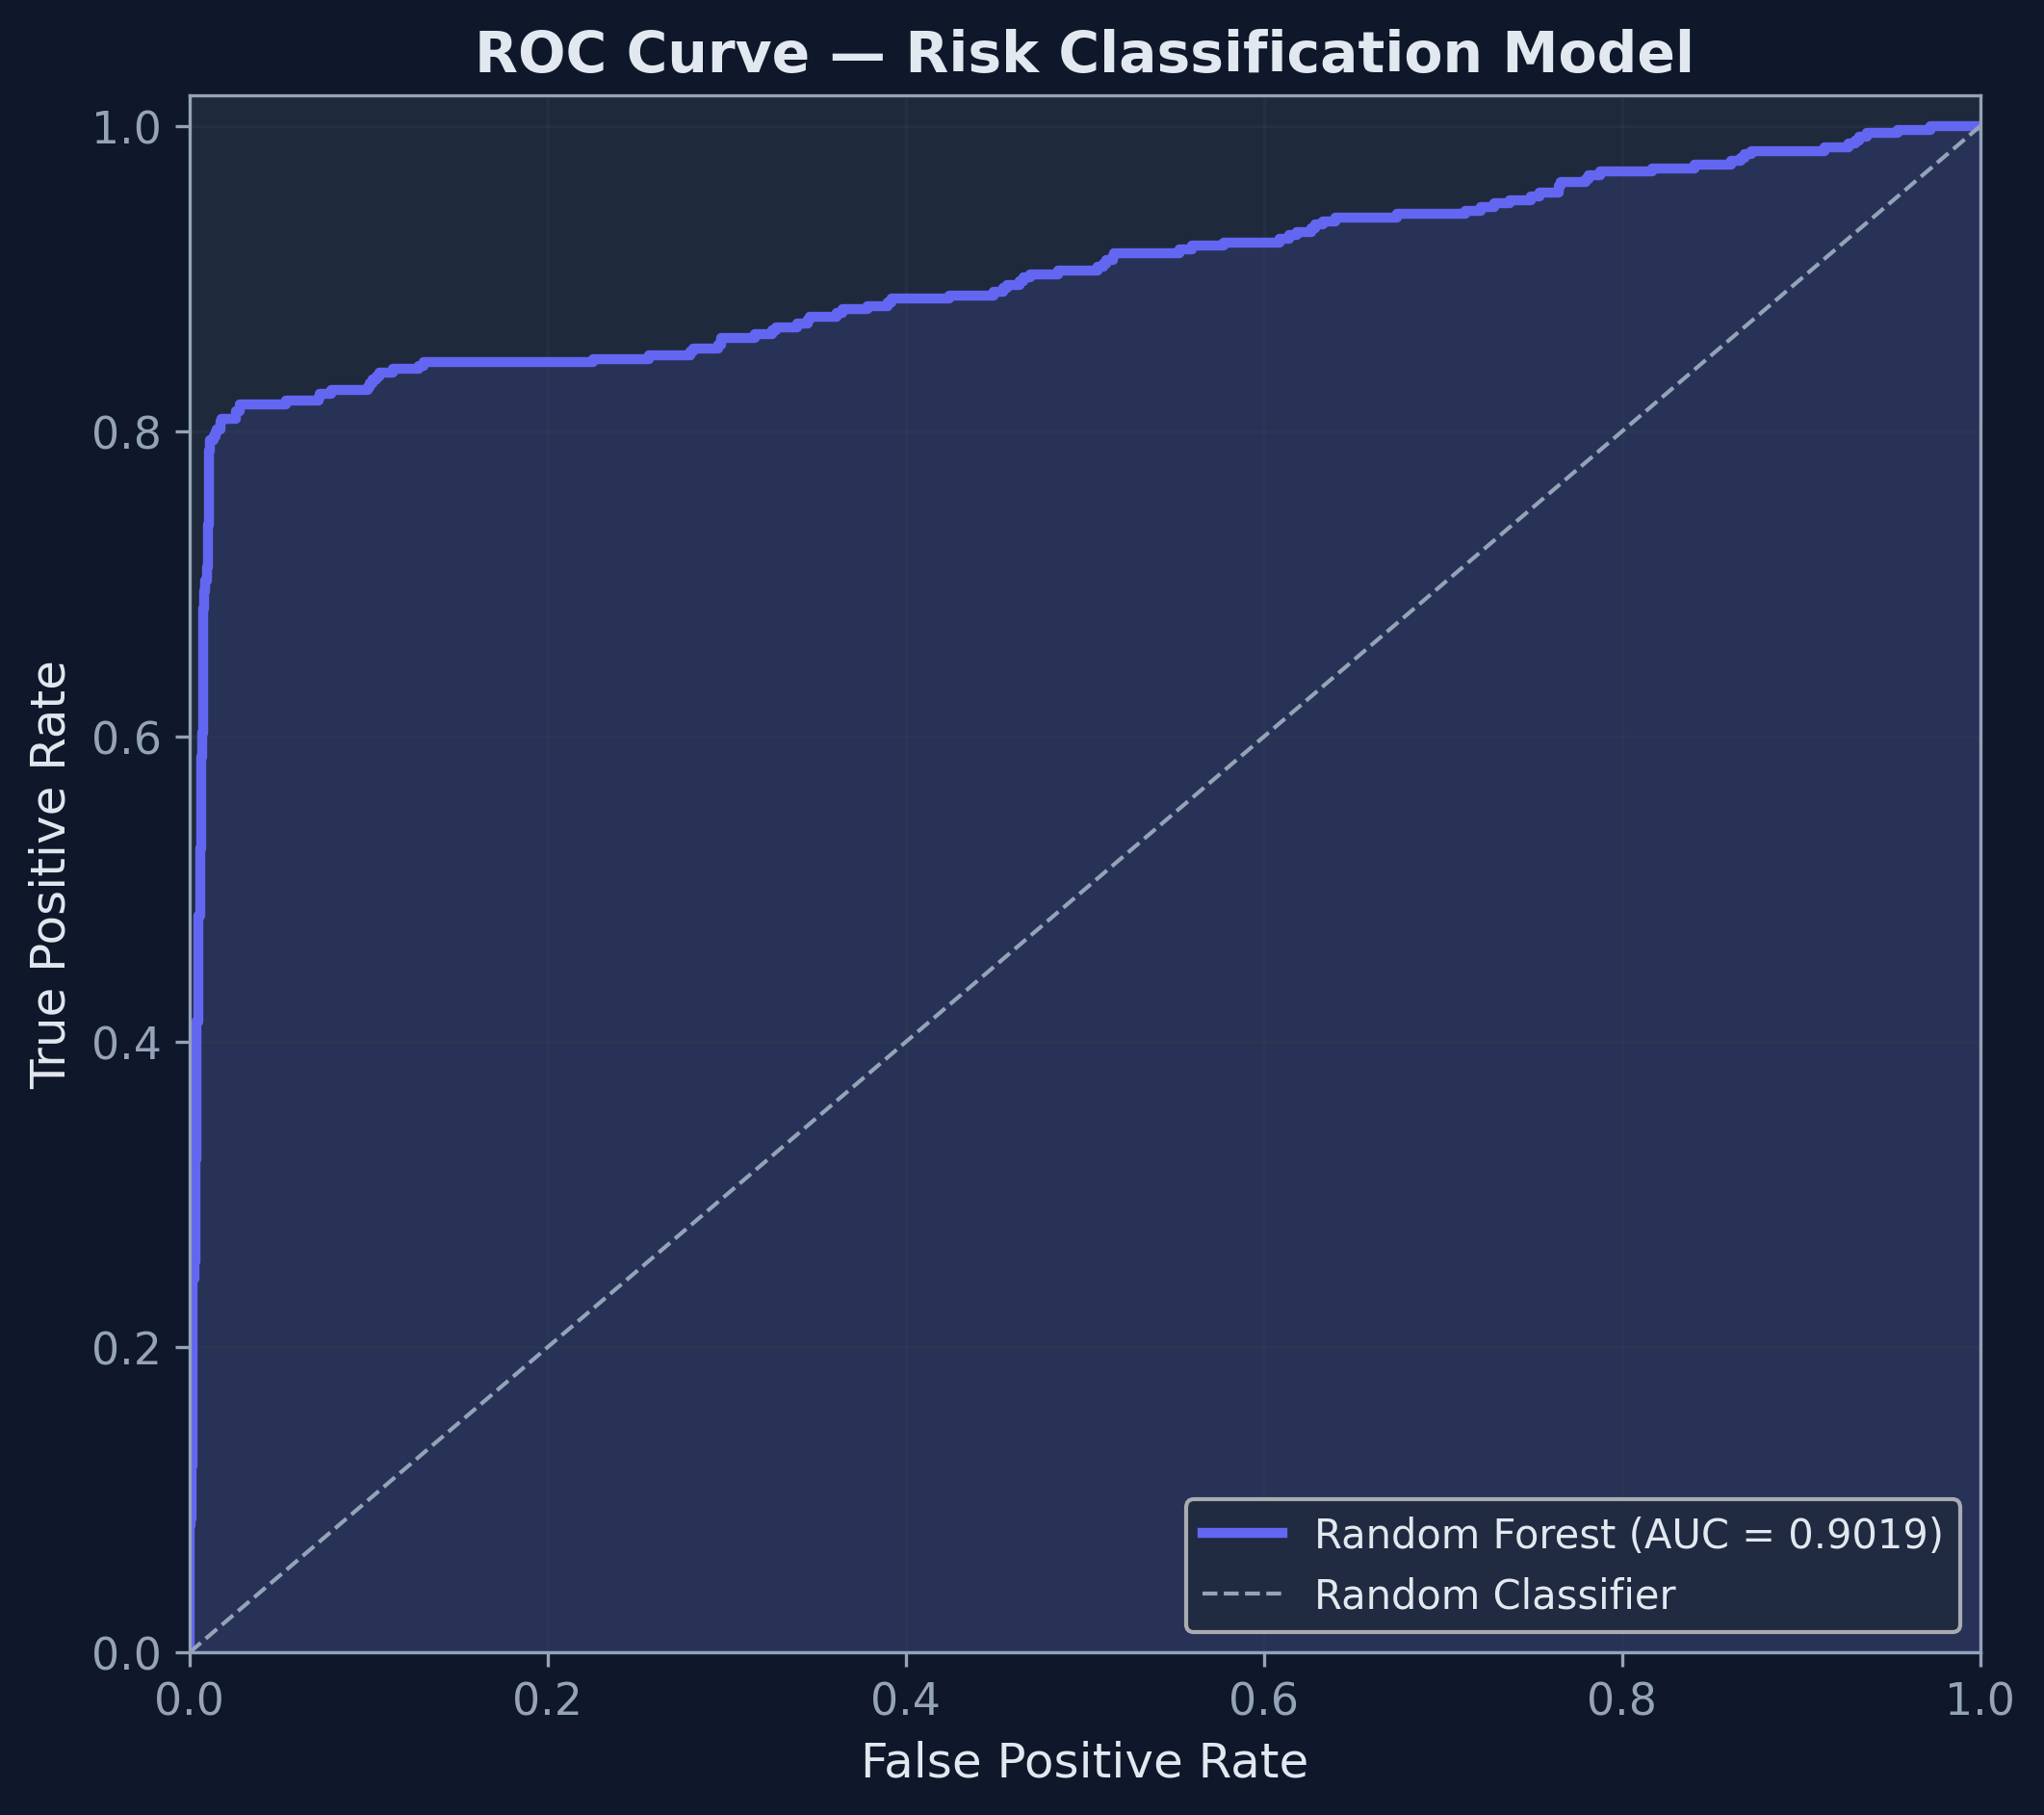
\includegraphics[width=\columnwidth]{evaluation/results/roc_curve.png}
\caption{ROC Curve (AUC = 0.9019).}
\label{fig:roc}
\end{figure}

\begin{figure*}[t]
\centering
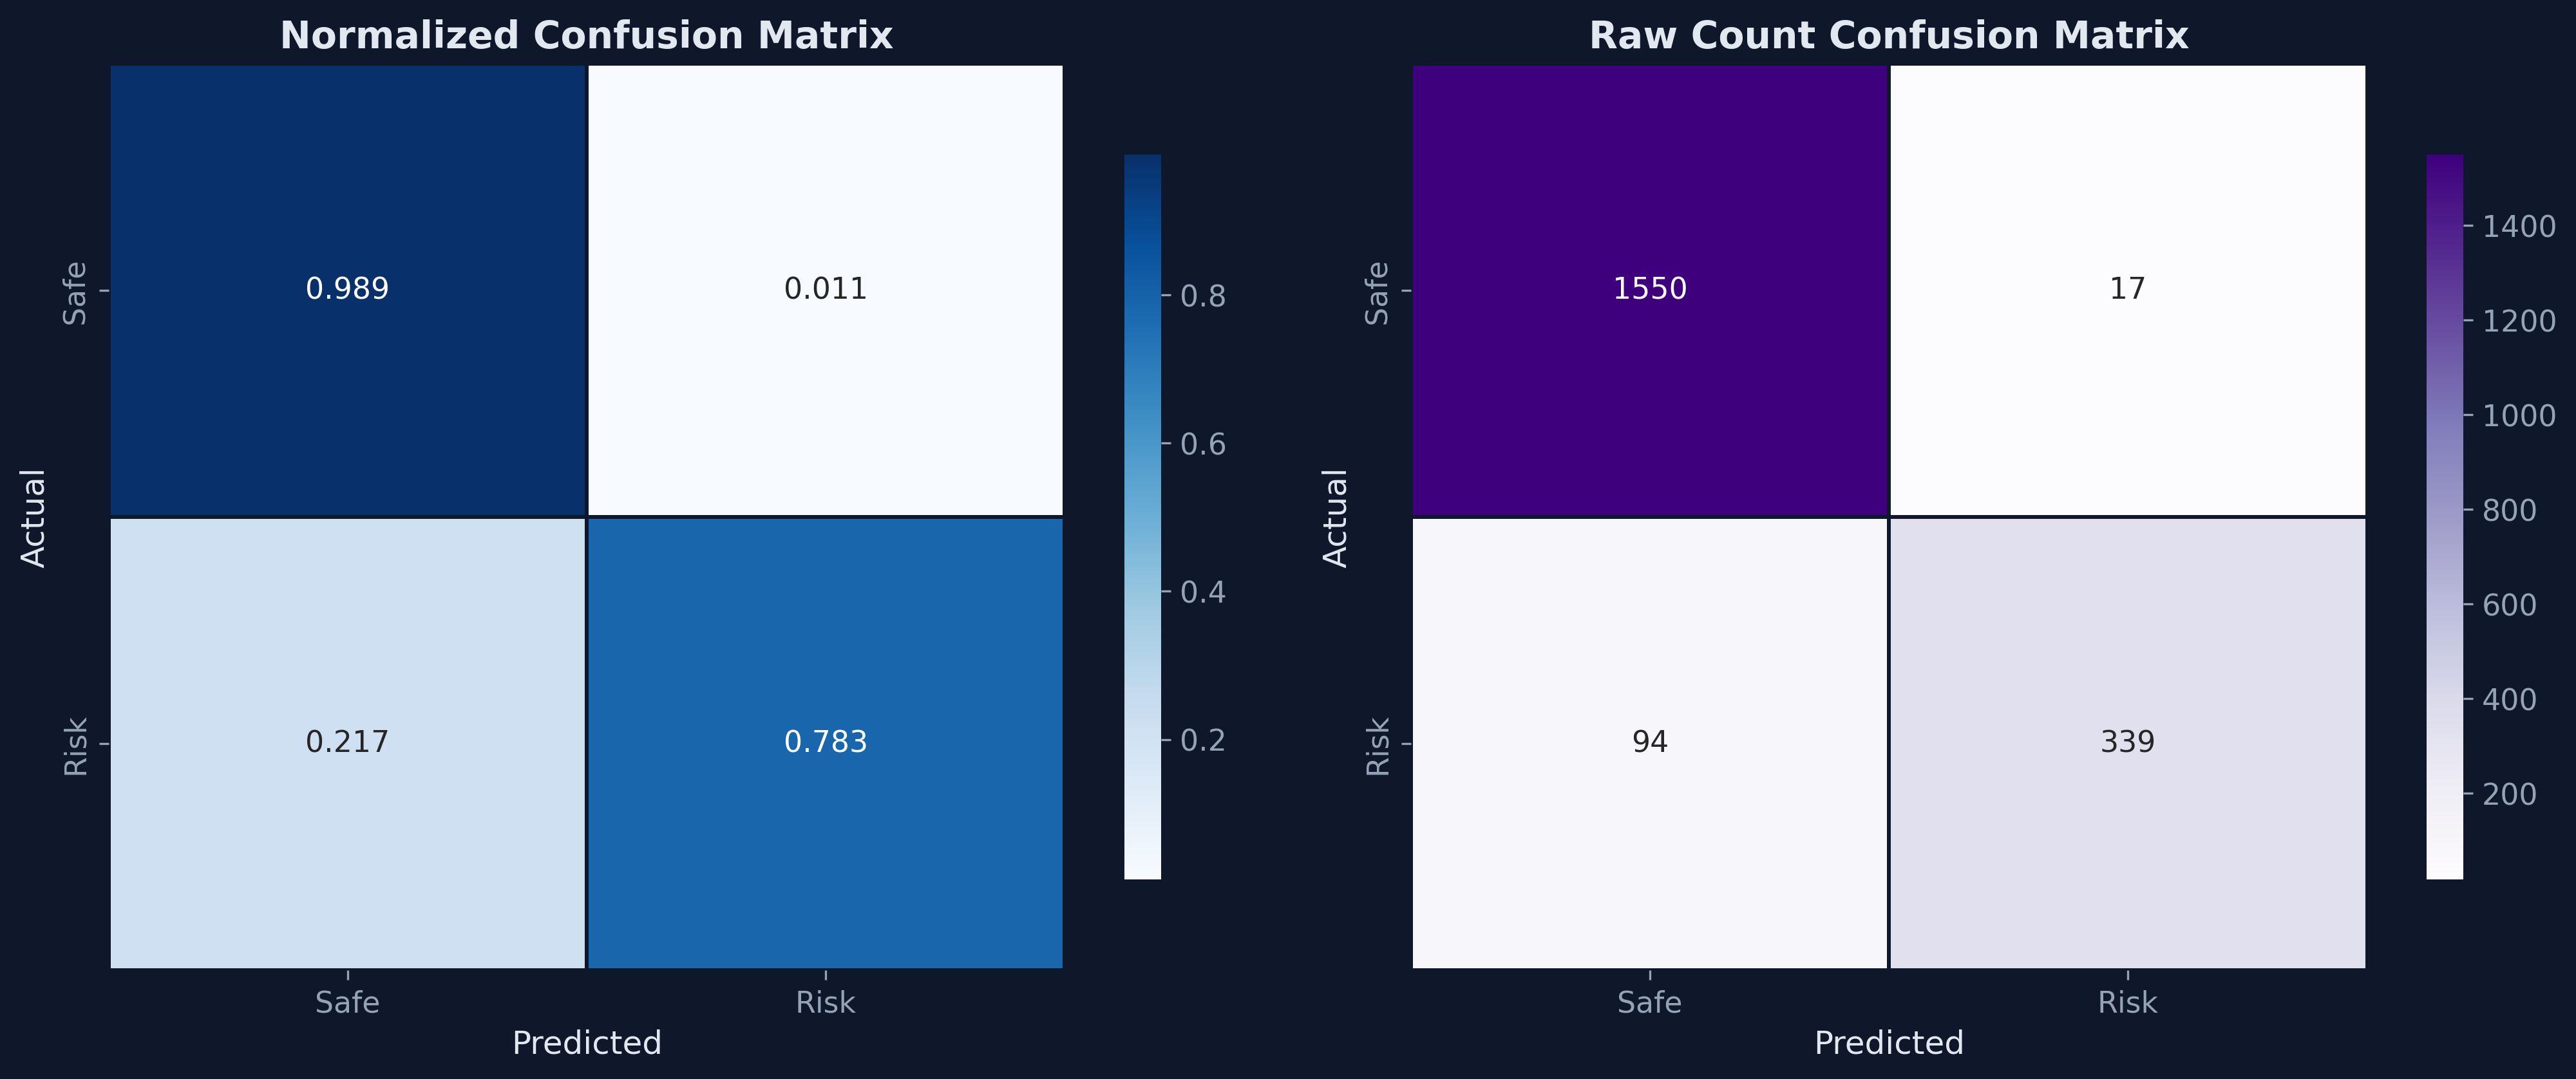
\includegraphics[width=\textwidth]{evaluation/results/confusion_matrix.png}
\caption{Normalized and raw-count confusion matrices.}
\label{fig:cm}
\end{figure*}

\subsection{Cross-Validation}
5-fold stratified cross-validation yields 94.91\% $\pm$ 0.27\% accuracy (10-fold: 95.00\% $\pm$ 0.35\%), confirming model generalizability with minimal variance across folds (Fig. \ref{fig:cv}).

\begin{figure}[t]
\centering
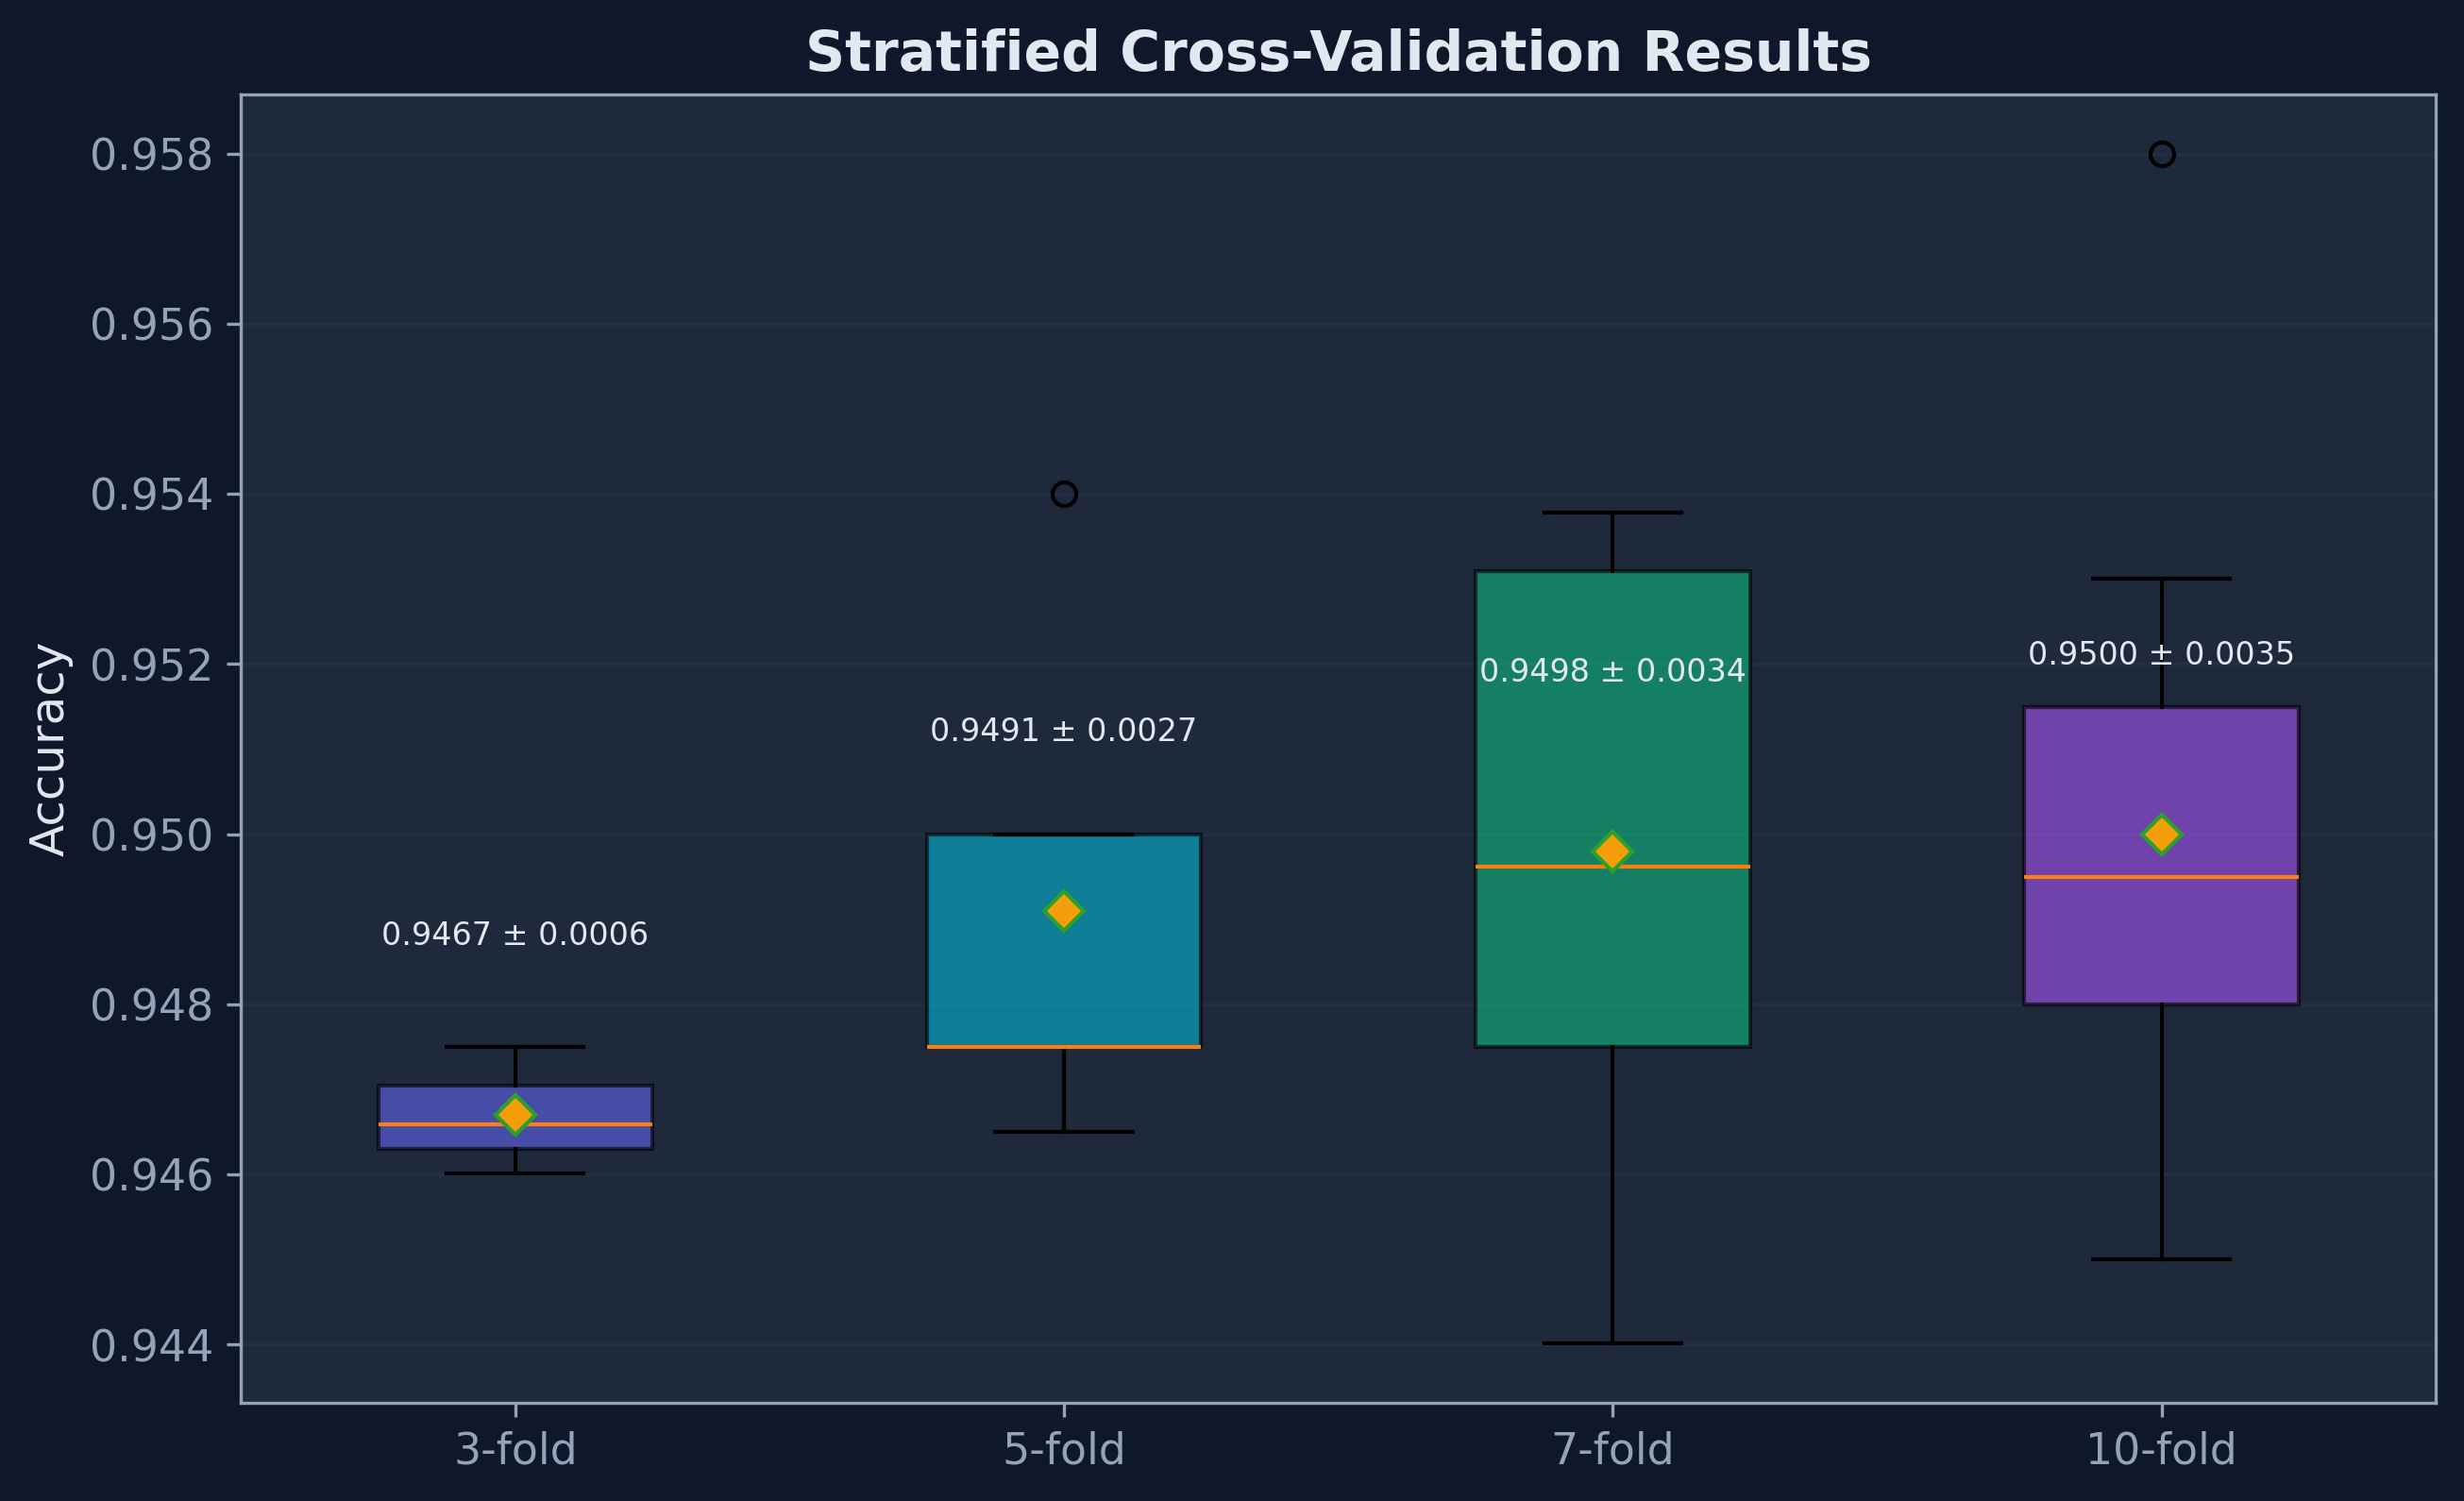
\includegraphics[width=\columnwidth]{evaluation/results/cross_validation.png}
\caption{Cross-Validation Stability.}
\label{fig:cv}
\end{figure}

\subsection{Feature Importance Analysis}
Feature importance analysis reveals that Threat Score (51.03\%) and Distance (22.50\%) collectively contribute 73.53\% of model decisions, aligning with cybersecurity domain knowledge \cite{freeman2016} (Fig. \ref{fig:fi}).

\begin{figure}[t]
\centering
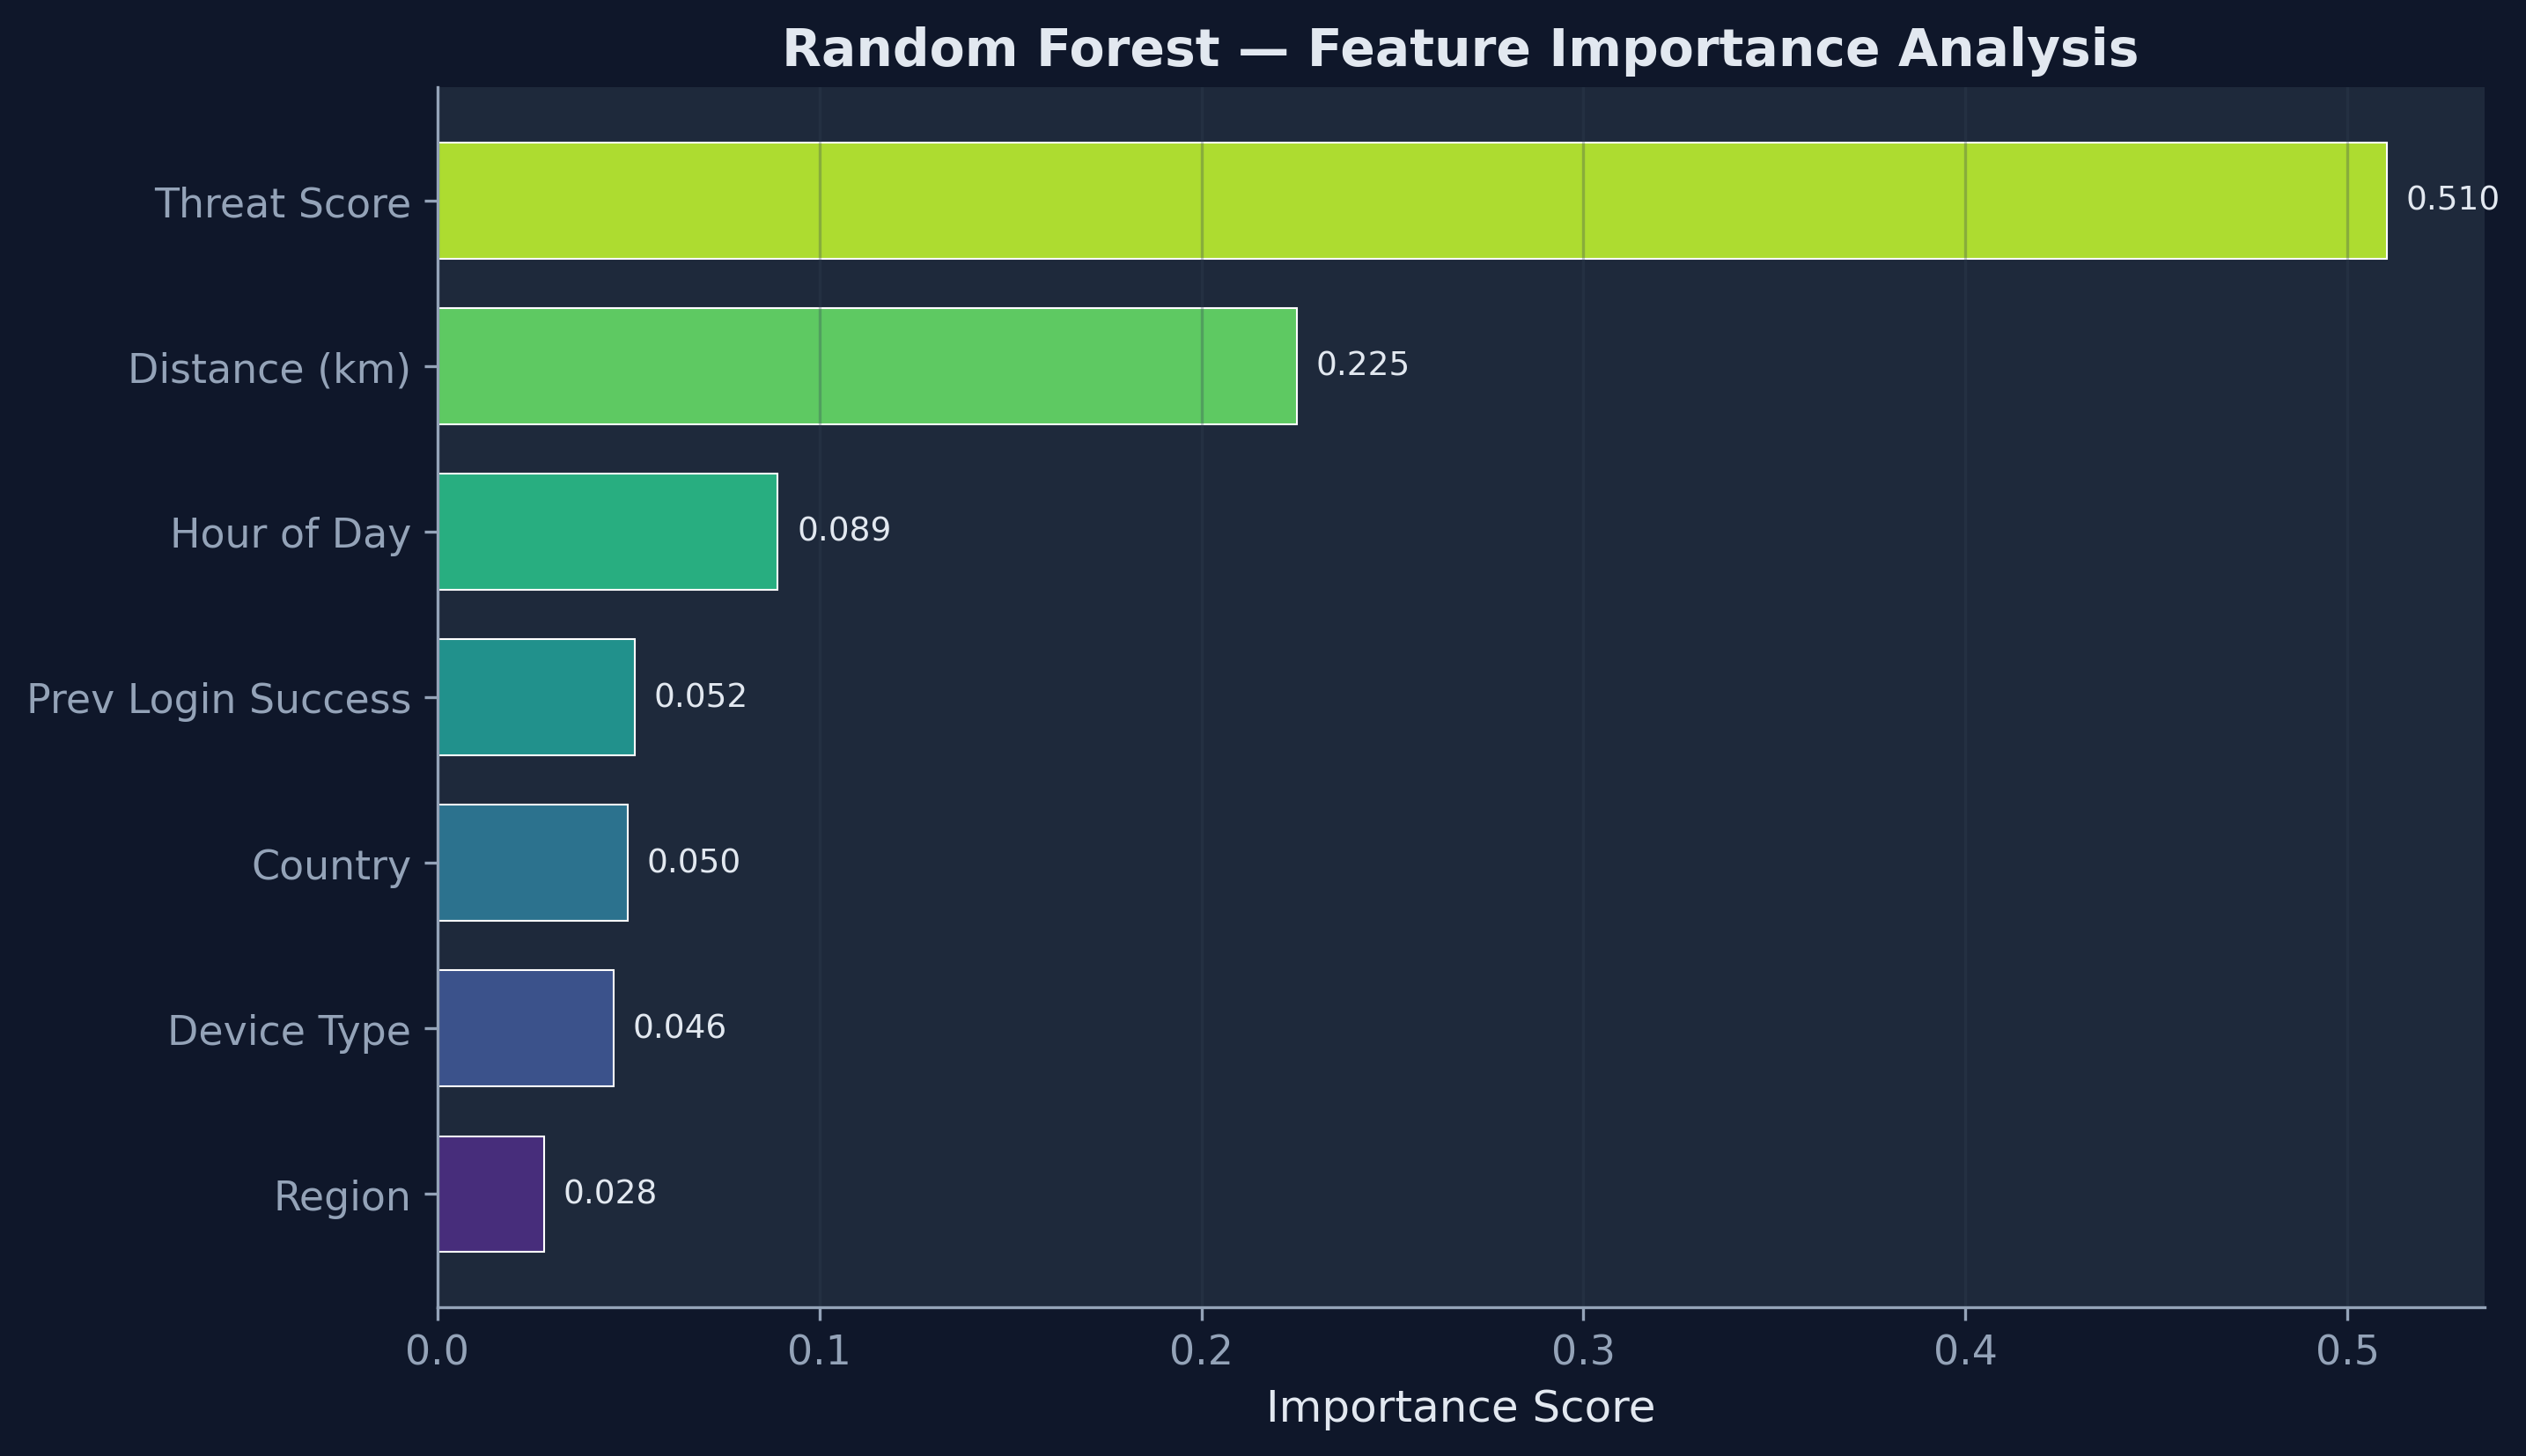
\includegraphics[width=\columnwidth]{evaluation/results/feature_importance.png}
\caption{Feature Importance Rankings.}
\label{fig:fi}
\end{figure}

\subsection{Feature-Ablation Study}\label{sec:ablation}
To quantify the model's dependence on each individual feature---and specifically to test the label-circularity concern noted in Section~\ref{sec:threat}---we perform a leave-one-feature-out ablation. For each of the seven features, we retrain the Random Forest on the remaining six and re-evaluate on the same 80/20 stratified split; we also train a single-feature model on Threat Score alone. Table~\ref{tab:ablation} reports the results.

\begin{table}[t]
\caption{Feature-Ablation Study (Leave-One-Out)}
\label{tab:ablation}
\centering
\setlength{\tabcolsep}{4pt}
\begin{tabular}{@{}lcccc@{}}
\toprule
Removed Feature & Acc & $\Delta$Acc & F1 & AUC \\
\midrule
\textit{None (full model)} & \textit{0.9445} & \textit{---} & \textit{0.8593} & \textit{0.9019} \\
Country & 0.9465 & $+$0.0020 & 0.8651 & 0.8972 \\
Region & 0.9465 & $+$0.0020 & 0.8654 & 0.9012 \\
Hour of Day & 0.9065 & $-$0.0380 & 0.7414 & 0.8882 \\
Device Type & 0.9330 & $-$0.0115 & 0.8241 & 0.9019 \\
Prev.\ Login & 0.9325 & $-$0.0120 & 0.8271 & 0.8950 \\
\textbf{Threat Score} & \textbf{0.8380} & $\boldsymbol{-}$\textbf{0.1065} & \textbf{0.4336} & \textbf{0.6624} \\
Distance & 0.8885 & $-$0.0560 & 0.6763 & 0.8392 \\
\midrule
\textit{Threat Score only} & \textit{0.8735} & --- & \textit{0.6053} & \textit{0.7686} \\
\bottomrule
\end{tabular}
\end{table}

Removing Threat Score causes the largest single-feature accuracy drop ($-$10.65~pp) and collapses F1 from 0.86 to 0.43, confirming that the model leans heavily on this feature. Because Threat Score is also one of the five rules used to generate training labels (Section~IV-B), its dominance is partly circular: the model has effectively learned to echo a label-construction rule. Conversely, Threat Score \textit{alone} reaches only 87.35\% accuracy versus 94.45\% for the full model, so the remaining features contribute a genuine 7.1~pp uplift not explained by circularity. Country and Region contribute negligibly; their removal actually \textit{improves} accuracy by 0.20~pp, suggesting mild overfitting to geographic noise. Distance ($-$5.60~pp) and Hour of Day ($-$3.80~pp) are the second- and third-most important features, consistent with the domain expectation that impossible-travel and temporal anomalies carry real signal.

\subsection{Model Comparison}
To justify model selection, we compare Random Forest against four baselines using identical data splits and evaluation protocols, summarized in Table \ref{tab:compare}.

Random Forest and XGBoost achieve comparable accuracy (94.45\% vs. 94.50\%) and F1 scores (0.8593 vs. 0.8622). The 0.05-point accuracy gap falls well within cross-validation variance and is not statistically meaningful; we therefore do \textit{not} claim Random Forest is the more accurate model. We select it instead for three practical reasons: (1) \textit{Interpretability}---native feature importance analysis enables security teams to audit risk decisions; (2) \textit{Cross-validation stability}---lowest CV variance ($\pm$0.0027 vs. $\pm$0.0034); (3) \textit{Hyperparameter robustness}---fewer tunable parameters reduces deployment risk. ROC comparison, a performance heatmap, and accuracy/F1/latency comparisons are shown in Fig. \ref{fig:roccmp}, Fig. \ref{fig:heatmap}, and Fig. \ref{fig:modelcmp}, respectively.

\begin{table}[t]
\caption{Classifier Comparison on Authentication Risk Detection}
\label{tab:compare}
\centering
\setlength{\tabcolsep}{4pt}
\begin{tabular}{@{}lccccc@{}}
\toprule
Model & Acc & F1 & ROC-AUC & CV (5-fold) & Inf (ms) \\
\midrule
\textbf{Random Forest} & \textbf{0.9445} & 0.8593 & 0.9019 & 0.9491$\pm$0.0027 & 53.99 \\
XGBoost (GBT) & 0.9450 & 0.8622 & 0.8986 & 0.9471$\pm$0.0034 & 0.19 \\
Logistic Regression & 0.8800 & 0.6712 & 0.8559 & 0.8696$\pm$0.0058 & 0.10 \\
SVM (RBF) & 0.9170 & 0.7816 & 0.9032 & 0.9141$\pm$0.0052 & 0.28 \\
K-Nearest Neighbors & 0.9030 & 0.7406 & 0.8719 & 0.9079$\pm$0.0053 & 19.61 \\
\bottomrule
\end{tabular}
\end{table}

\begin{figure}[t]
\centering
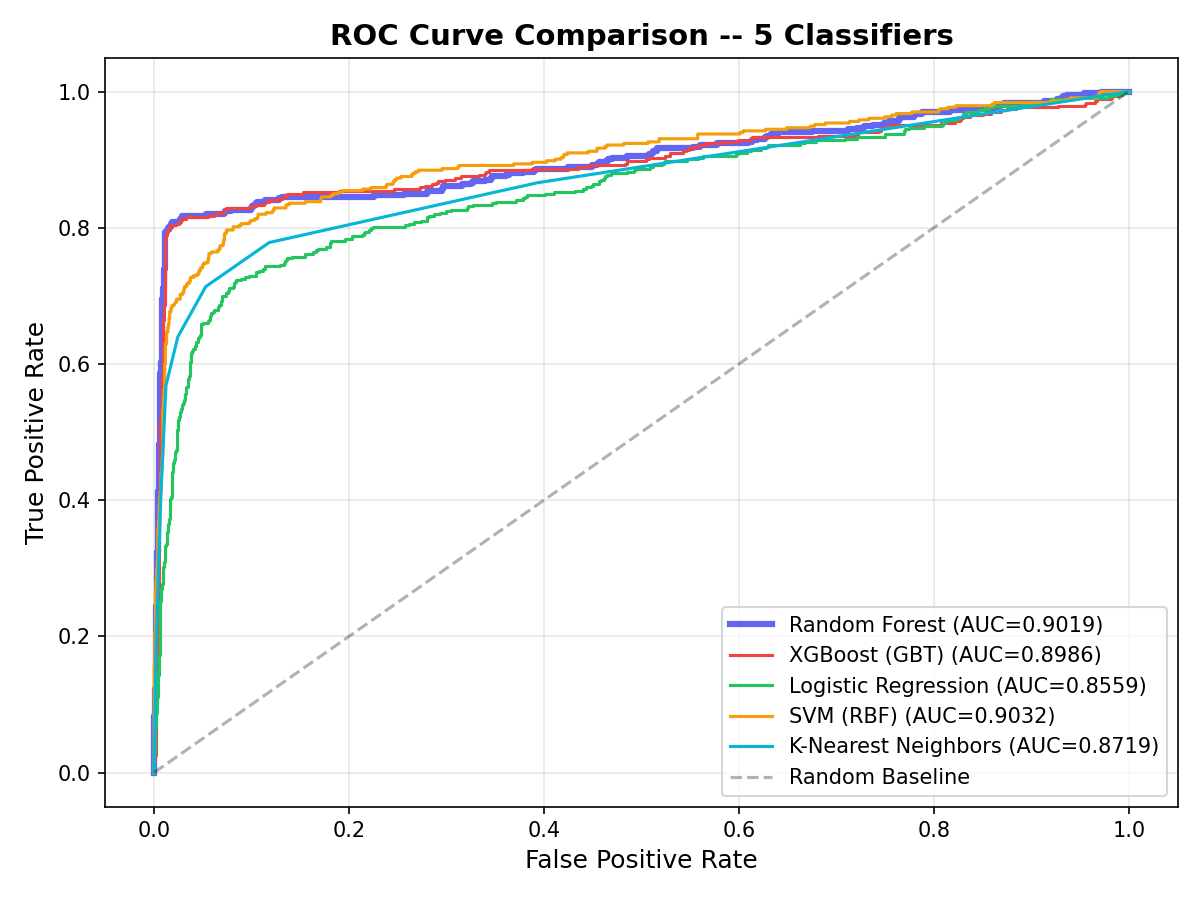
\includegraphics[width=\columnwidth]{evaluation/results/model_comparison_roc.png}
\caption{ROC Curve Comparison---5 Classifiers.}
\label{fig:roccmp}
\end{figure}

\begin{figure}[t]
\centering
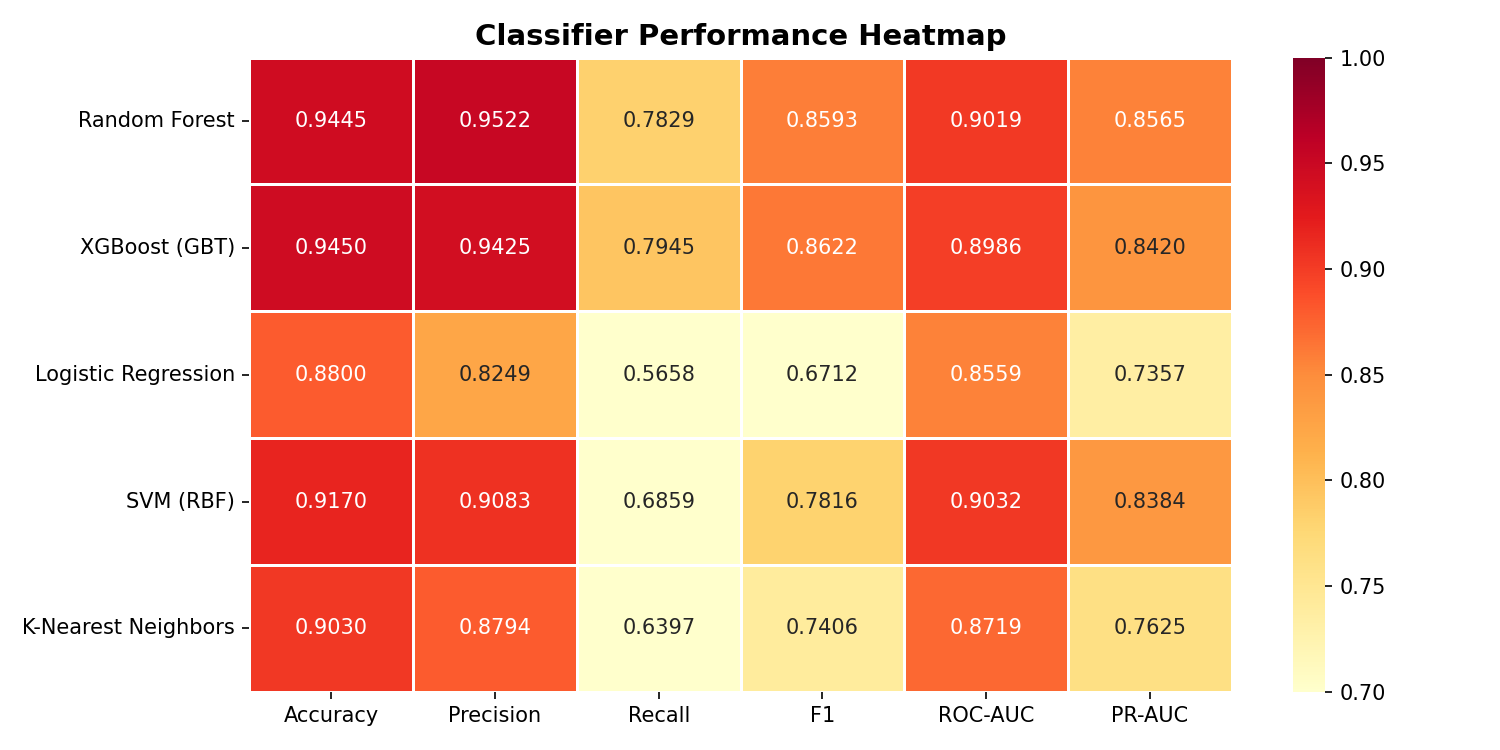
\includegraphics[width=\columnwidth]{evaluation/results/model_comparison_heatmap.png}
\caption{Classifier Performance Heatmap.}
\label{fig:heatmap}
\end{figure}

\begin{figure*}[t]
\centering
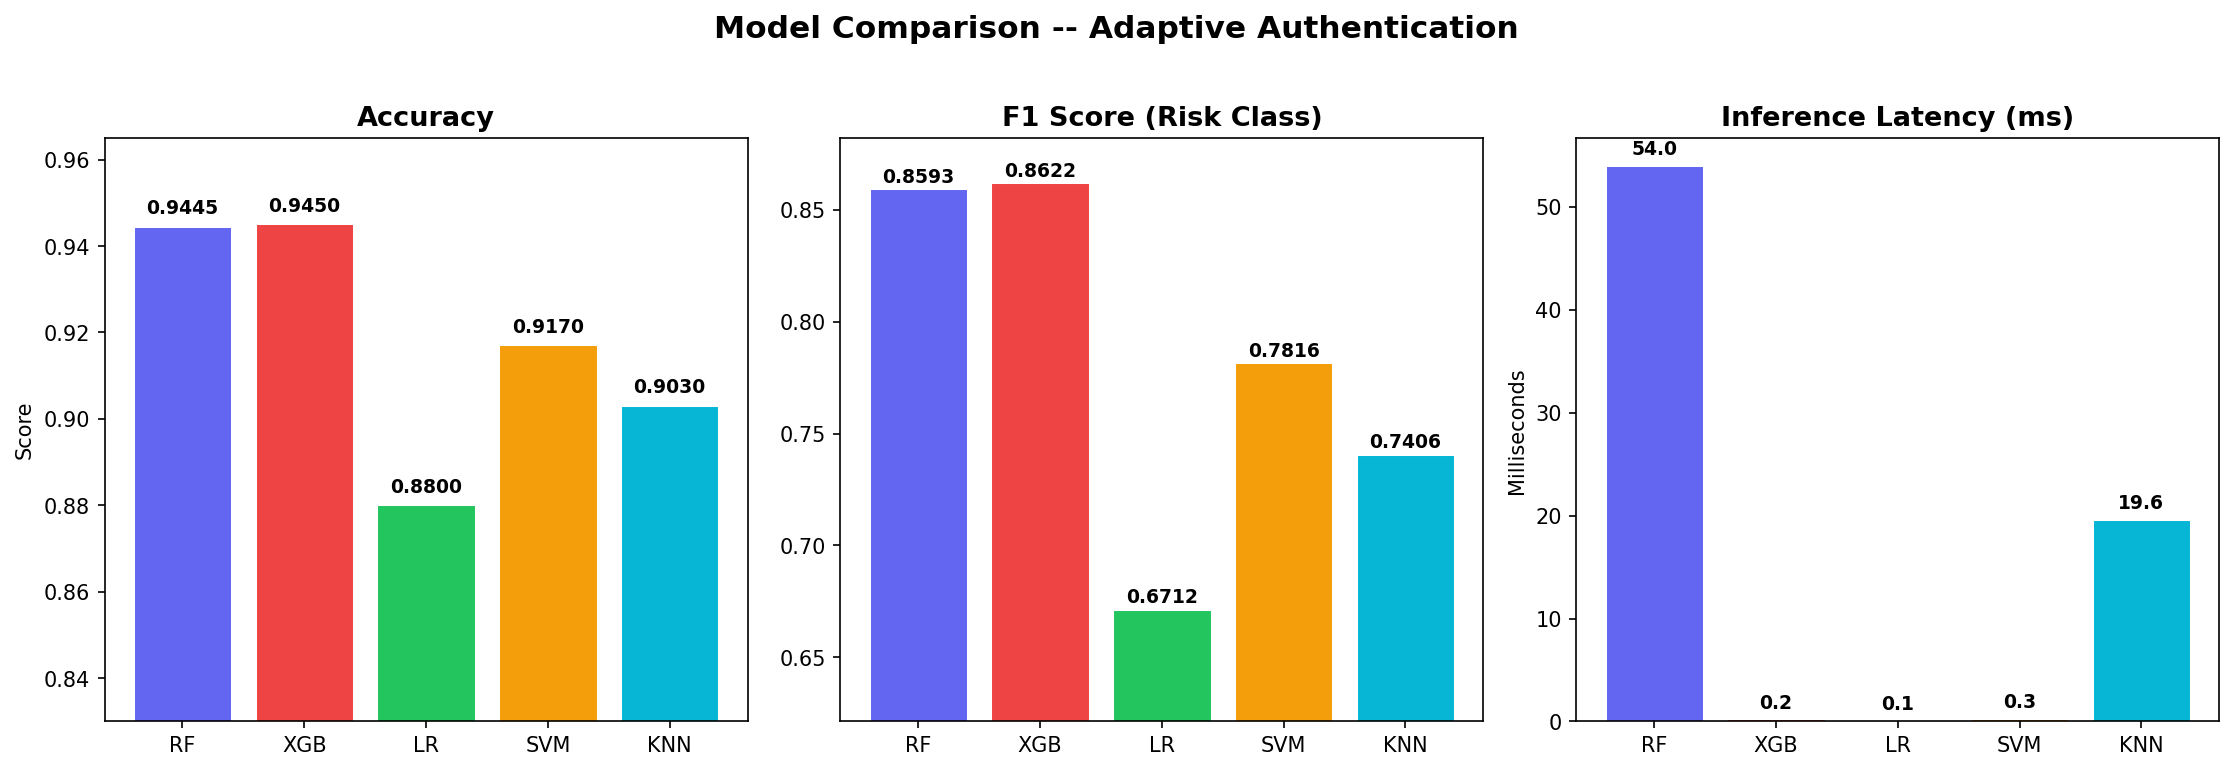
\includegraphics[width=\textwidth]{evaluation/results/model_comparison_bars.png}
\caption{Model Comparison---Accuracy, F1, Latency.}
\label{fig:modelcmp}
\end{figure*}

\subsection{Security Evaluation}\label{sec:seceval}
We evaluate security efficacy against 1,500 adversarial scenarios across 21 attack profiles categorized into three risk tiers, as reported in Table \ref{tab:security}.

At the balanced threshold (0.5), the system achieves precision $= 1.0$ with zero false positives on the synthetic legitimate set, meaning no legitimate user in our evaluation was wrongly blocked. The false negative rate of 14.13\% affects only medium-risk scenarios, where users receive MFA challenges---a proportional response. Per-category detection and mean risk scores are visualized in Fig. \ref{fig:attack}.

\begin{table}[t]
\caption{Security Evaluation by Risk Category}
\label{tab:security}
\centering
\begin{tabular}{@{}lcccc@{}}
\toprule
Category & Scenarios & Detected & Rate & Avg Score \\
\midrule
High-Risk & 500 & 500 & 100\% & 0.9362 \\
Medium-Risk & 250 & 144 & 57.6\% & 0.4767 \\
Legitimate & 750 & 0 & 0\% FP & 0.0712 \\
\bottomrule
\end{tabular}
\end{table}

\begin{figure*}[t]
\centering
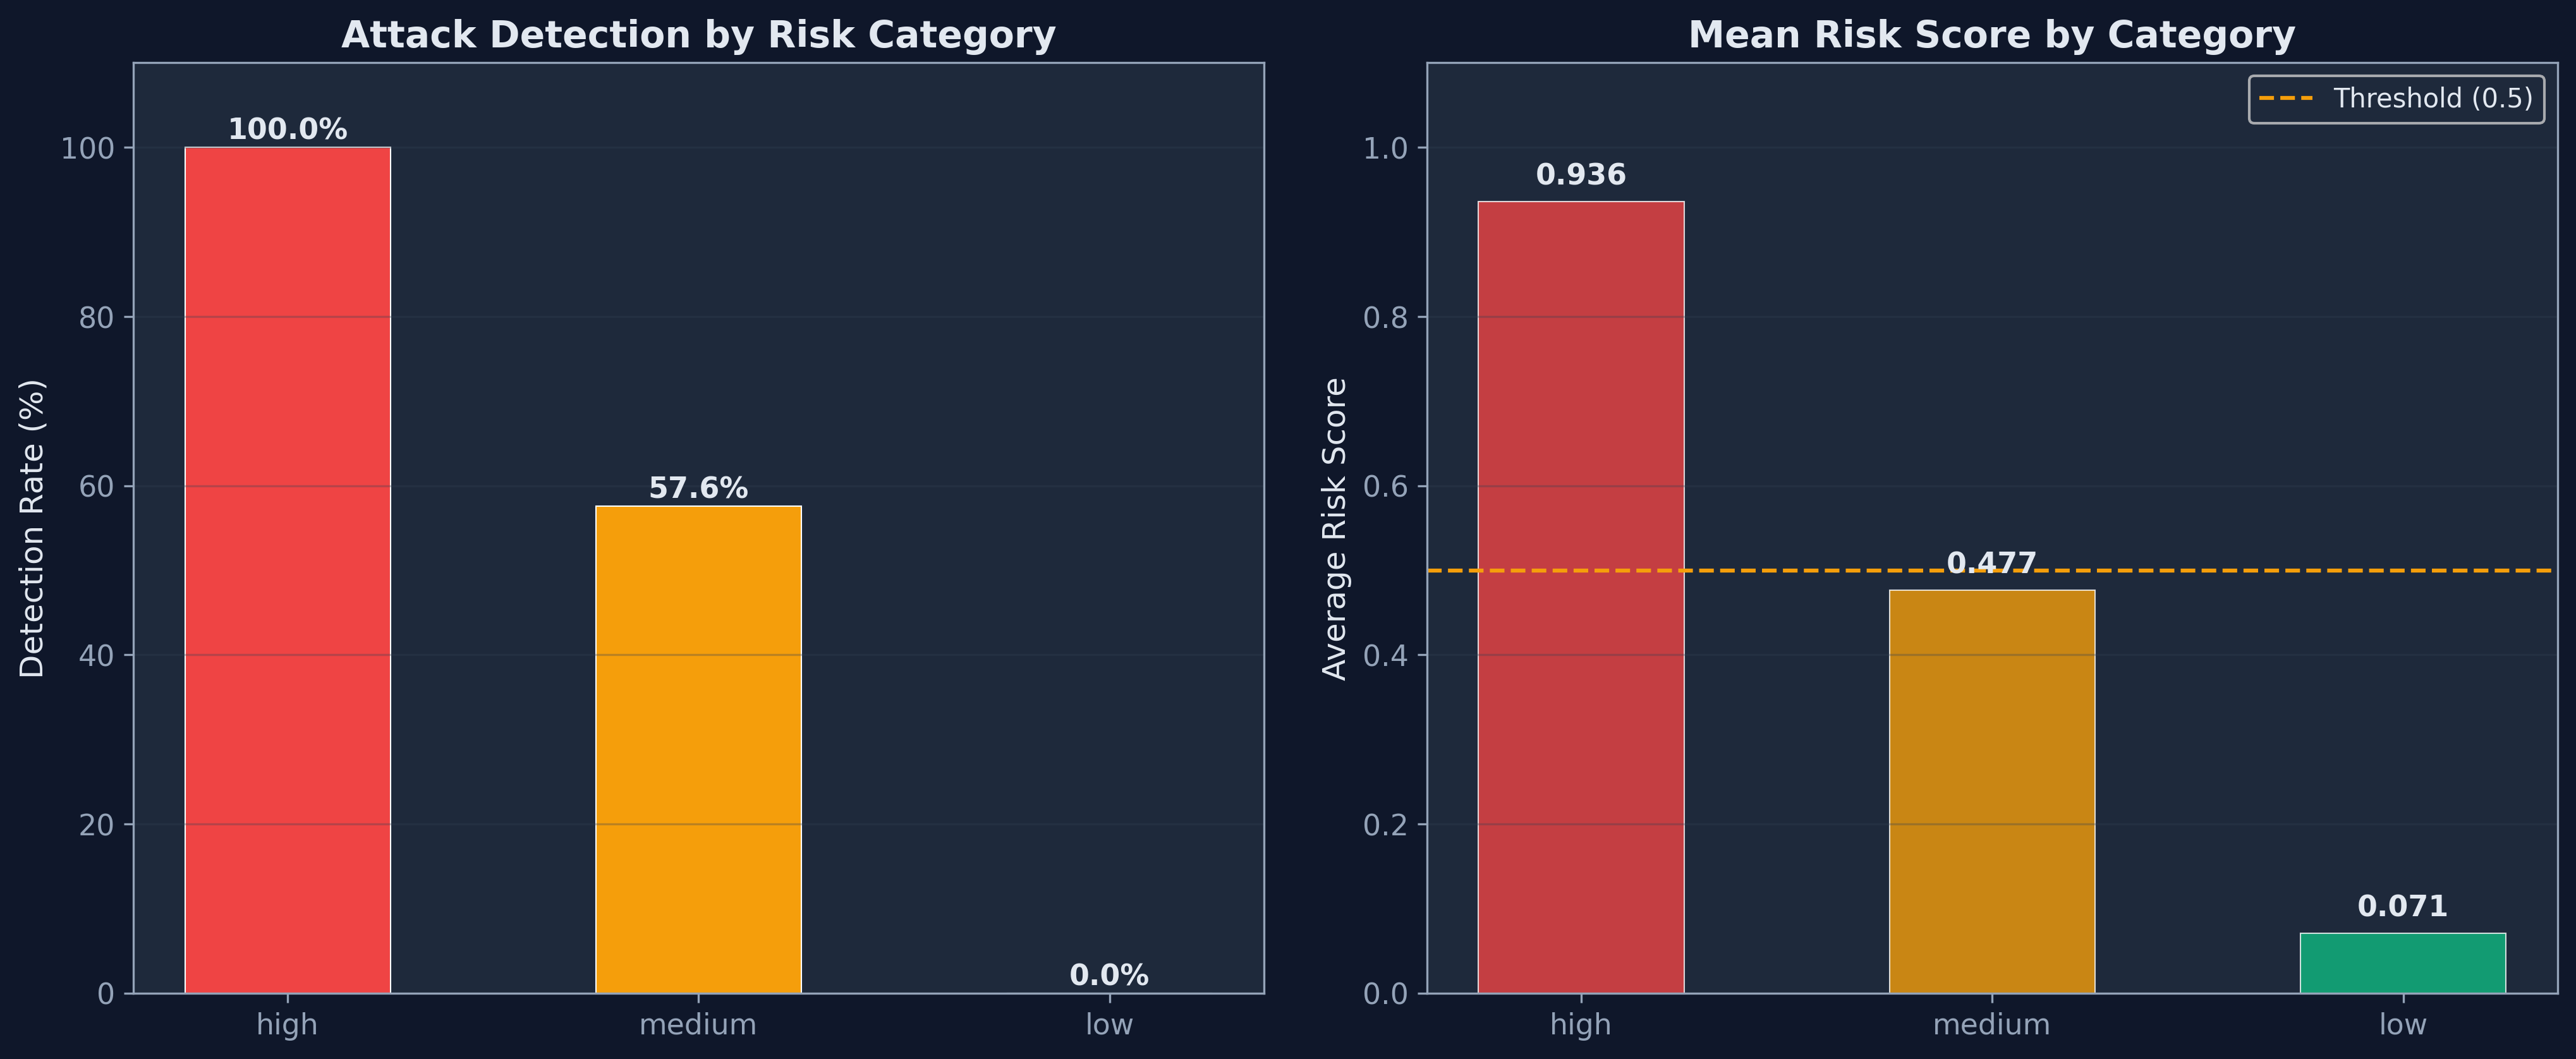
\includegraphics[width=\textwidth]{evaluation/results/security_detection.png}
\caption{Attack Detection by Profile.}
\label{fig:attack}
\end{figure*}

\subsection{Adaptive-Adversary Evasion Cost}
The rule-generated evaluation above measures detection against a \textit{fixed} attack distribution and, because those same rules generate the training labels, cannot establish robustness against a \textit{strategic} adversary. We therefore introduce an evasion-cost analysis that probes the decision boundary directly. Starting from every attacker the model already BLOCKs ($r \ge 0.7$), we search for the minimum-cost set of feature edits---restricted to the features the adversary controls under the threat model of Section~\ref{sec:threat}---that pushes the risk score below the block threshold. Each mutable feature is assigned a cost reflecting the real capability its modification requires (Table~\ref{tab:evcost}); \textit{Prev.\ Login} is treated as immutable, since an attacker cannot fabricate the victim's account history.

We report three quantities: the \textit{evasion rate} (fraction of blocked attackers able to reach $r < 0.7$), the \textit{mean evasion cost} (summed weights of edited features), and the \textit{cheapest-lever distribution} (how often each feature appears in a minimal evasion set). The last is the most diagnostic: a feature that dominates minimal evasion sets is the one the defense actually rests on.

\begin{table}[t]
\caption{Attacker Cost Model for Mutable Features}
\label{tab:evcost}
\centering
\begin{tabular}{@{}lll@{}}
\toprule
Feature & Required capability & Cost \\
\midrule
Hour of Day & Time the login attempt & 1 \\
Device Type & Spoof user-agent & 1 \\
Country & VPN via benign country & 2 \\
Region & VPN via benign region & 2 \\
Distance & VPN endpoint near victim & 3 \\
Threat Score & Acquire clean (unflagged) IP & 3 \\
Prev. Login & Cannot fake account history & $\infty$ \\
\bottomrule
\end{tabular}
\end{table}

Table~\ref{tab:evasion} reports evasion-cost results computed on the full set of 1{,}737 blocked samples ($r \ge 0.7$) in our synthetic benchmark. The finding is sobering and, we argue, more informative than the near-perfect detection of Section~\ref{sec:seceval}: every blocked attacker can evade the block by changing on average just 1.03 features. Threat Score is the dominant lever (52.5\% of minimal evasion sets), followed by Hour of Day (21.2\%) and Distance (17.0\%). This is consistent with the ablation findings of Section~\ref{sec:ablation}: the model's reliance on Threat Score---which is attacker-controllable via clean, unflagged IP infrastructure---means the system's apparent robustness largely collapses to IP reputation. This simultaneously explains the circular high detection rate and identifies the concrete design remedy: robustness requires features that are jointly costly to spoof, motivating the behavioral biometrics discussed in our future work.

\begin{table}[t]
\caption{Evasion-Cost Results (1{,}737 Blocked Samples)}
\label{tab:evasion}
\centering
\begin{tabular}{@{}lc@{}}
\toprule
Metric & Value \\
\midrule
Evasion rate (reach $r < 0.7$) & 100.0\% \\
Mean evasion cost & 2.47 \\
Mean features changed & 1.03 \\
Dominant lever --- Threat Score & 52.5\% \\
Second lever --- Hour of Day & 21.2\% \\
Third lever --- Distance & 17.0\% \\
Resistant (no evasion found) & 0.0\% \\
\bottomrule
\end{tabular}
\end{table}

\subsection{Threshold Sensitivity}
Table \ref{tab:threshold} and Fig. \ref{fig:threshold} characterize the trade-off between accuracy, precision, recall, and F1 across decision thresholds.

\begin{table}[t]
\caption{Threshold Sensitivity Analysis}
\label{tab:threshold}
\centering
\begin{tabular}{@{}ccccc@{}}
\toprule
Threshold & Accuracy & Precision & Recall & F1 \\
\midrule
0.2 & 0.9300 & 0.8530 & 0.8176 & 0.8349 \\
0.3 & 0.9440 & 0.9303 & 0.8014 & 0.8610 \\
0.4 & 0.9450 & 0.9425 & 0.7945 & 0.8622 \\
\textbf{0.5} & \textbf{0.9445} & \textbf{0.9522} & \textbf{0.7829} & \textbf{0.8593} \\
0.6 & 0.9405 & 0.9511 & 0.7644 & 0.8476 \\
0.7 & 0.9335 & 0.9518 & 0.7298 & 0.8261 \\
0.8 & 0.9225 & 0.9603 & 0.6697 & 0.7891 \\
\bottomrule
\end{tabular}
\end{table}

\begin{figure}[t]
\centering
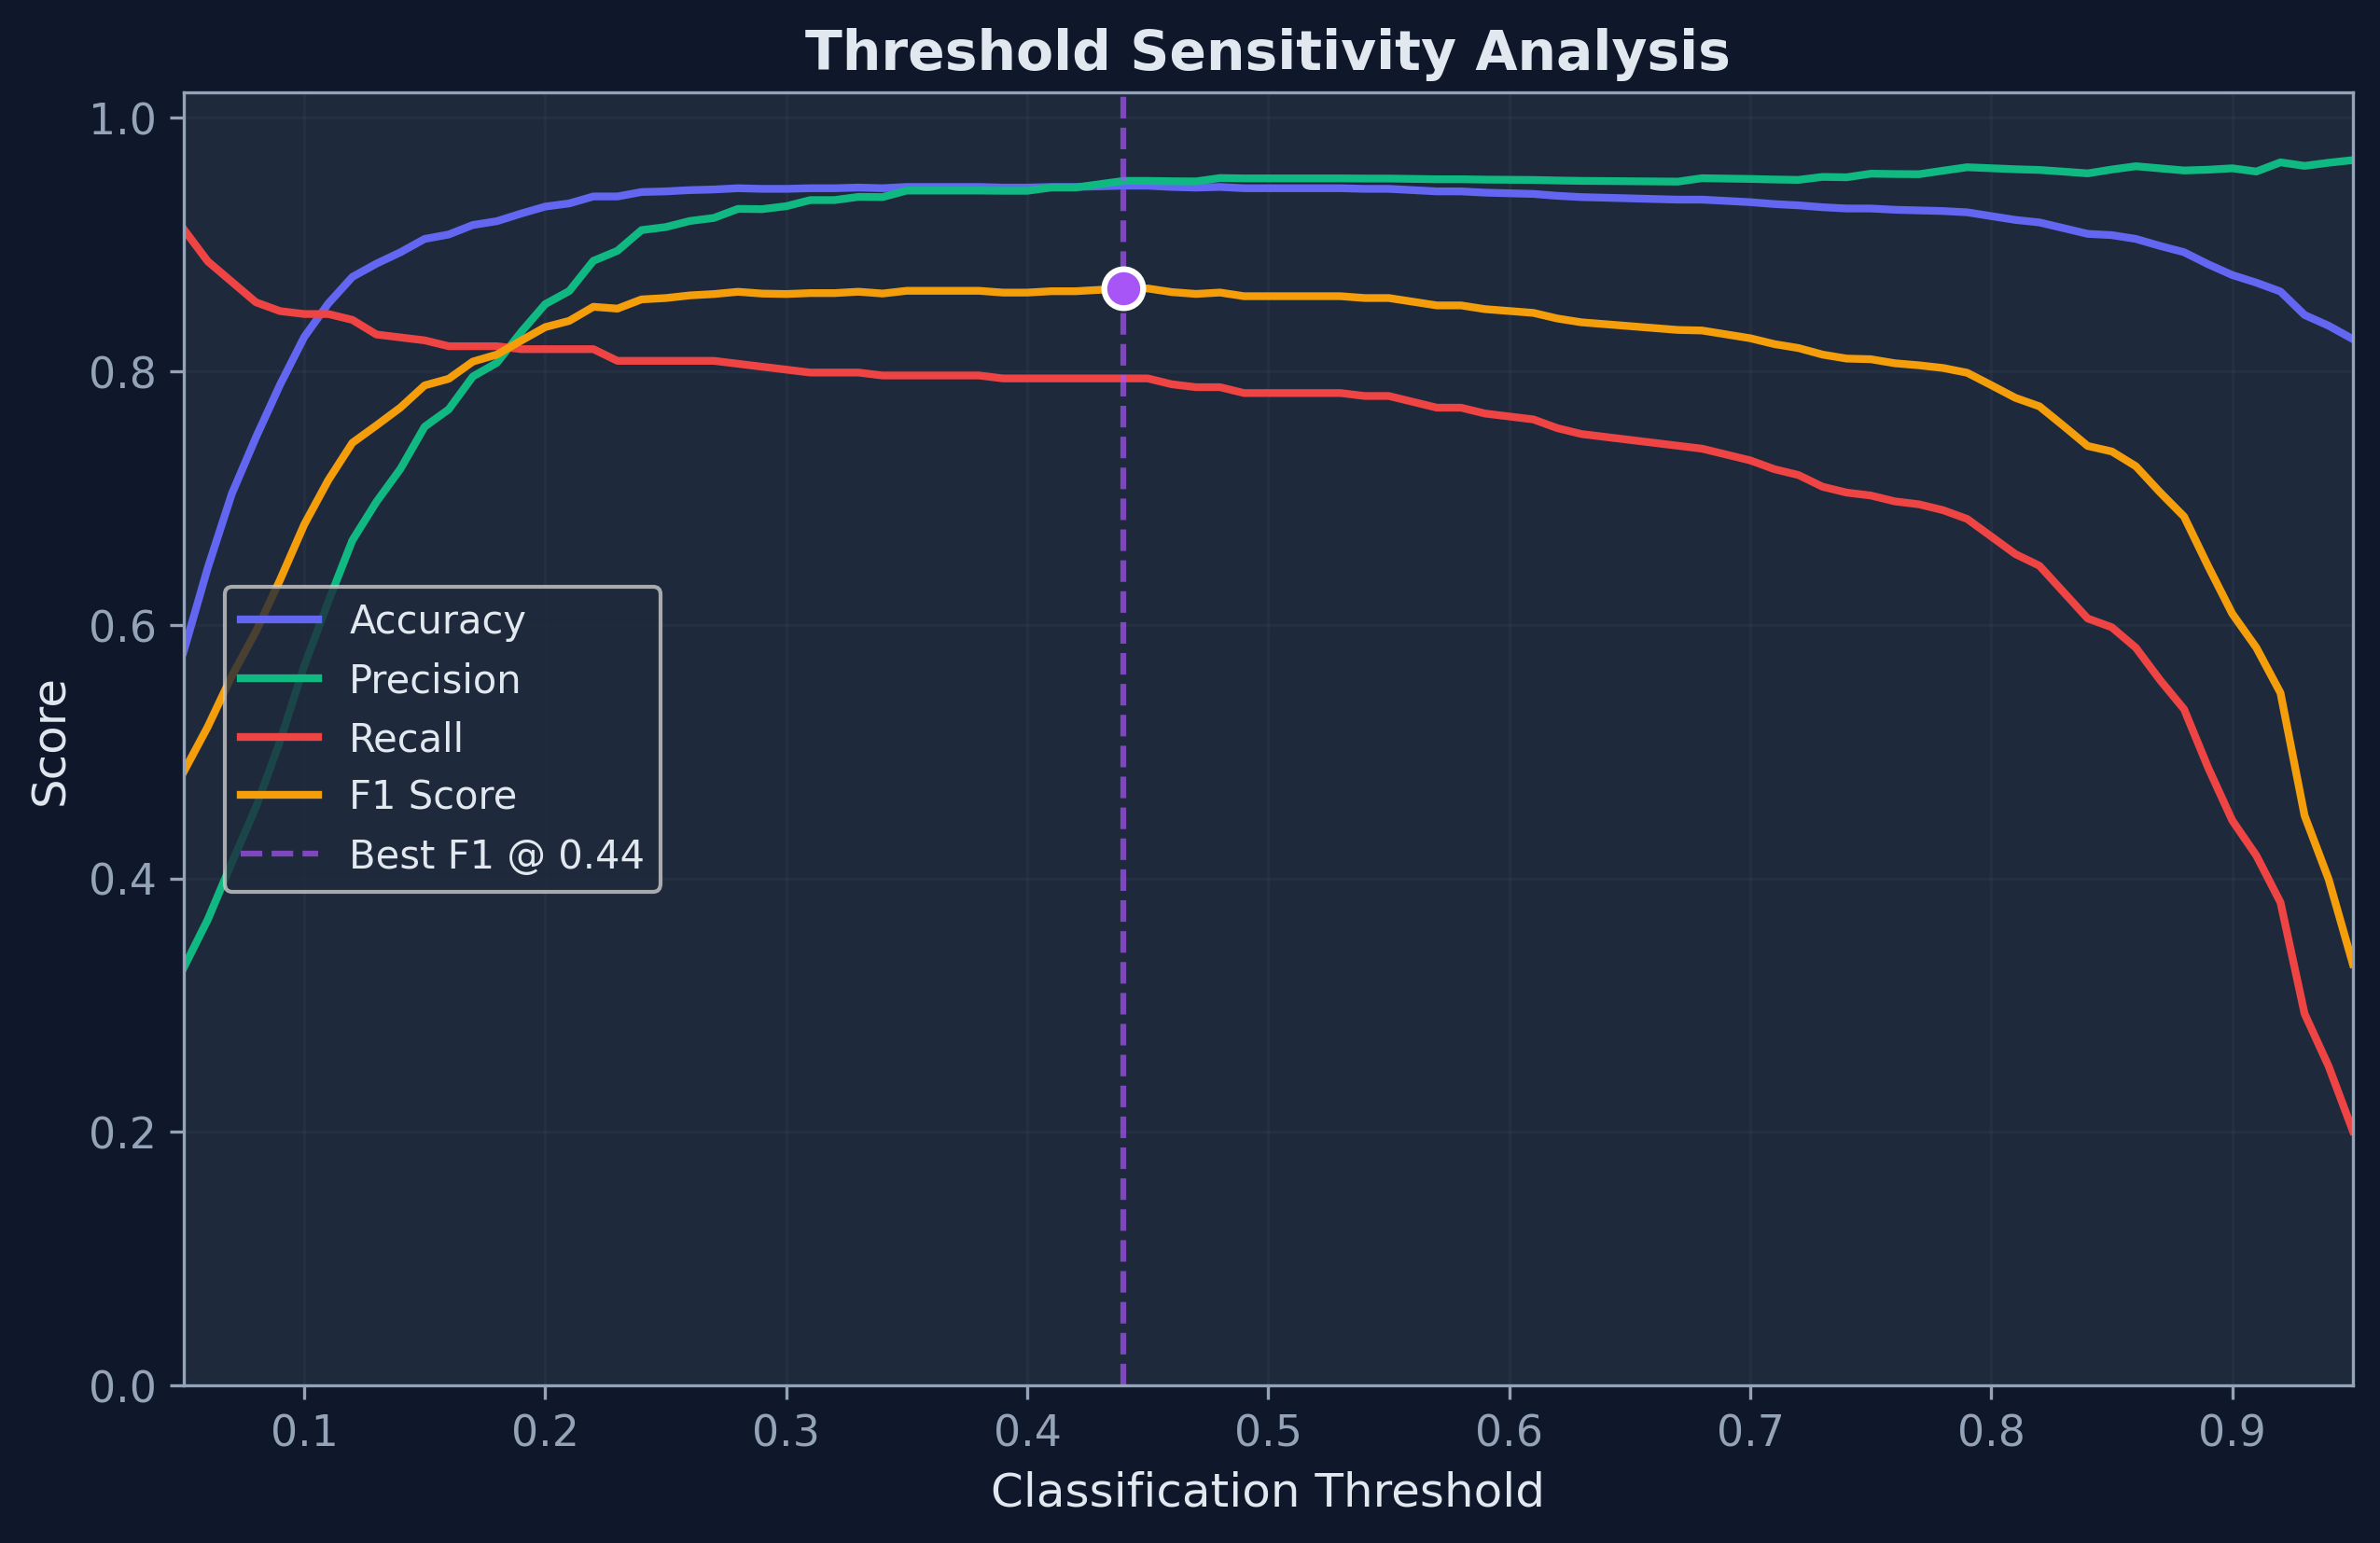
\includegraphics[width=\columnwidth]{evaluation/results/threshold_analysis.png}
\caption{Threshold Sensitivity Curves.}
\label{fig:threshold}
\end{figure}

\subsection{Performance Benchmarks}\label{sec:latency}
The system achieves a median inference latency of 43 ms (p95: 60 ms, p99: 70 ms), well within the 100 ms threshold for real-time authentication; the full distribution is shown in Fig. \ref{fig:latency}. The higher per-model value reported in Table \ref{tab:compare} (53.99 ms for Random Forest) is the \textit{mean} latency, which exceeds the median because the distribution is right-skewed.

\begin{figure}[t]
\centering
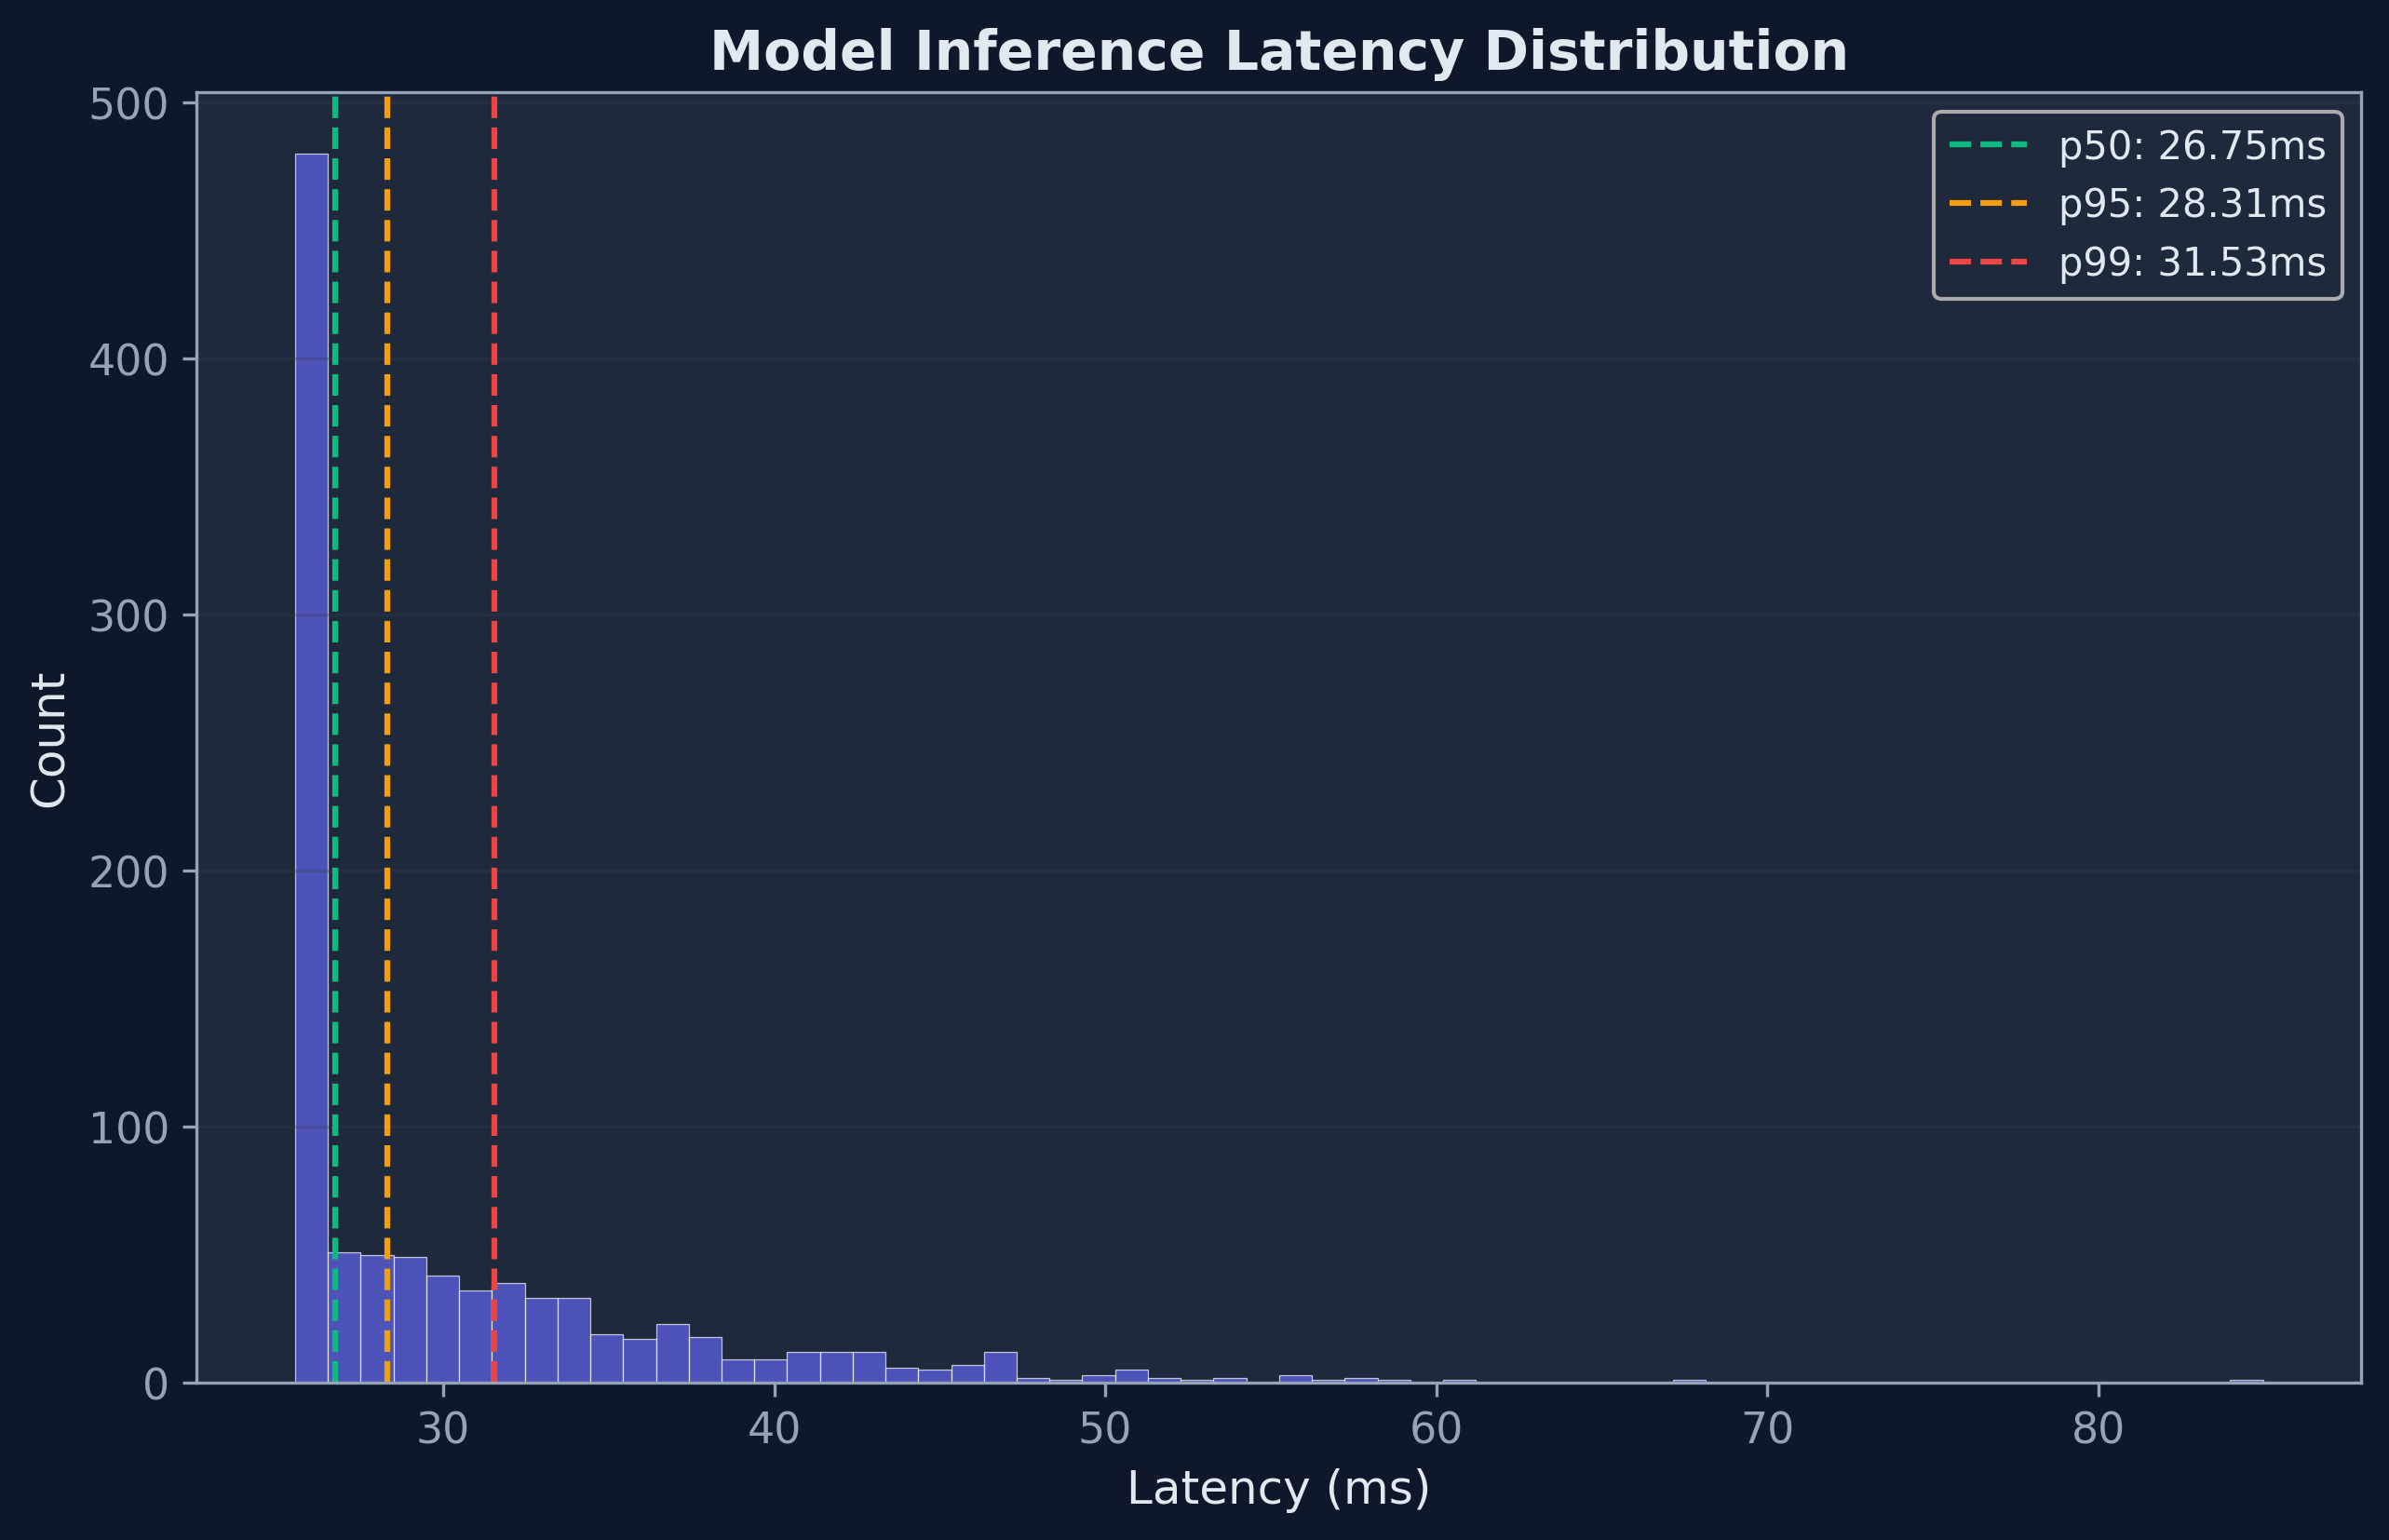
\includegraphics[width=\columnwidth]{evaluation/results/latency_distribution.png}
\caption{Inference Latency Distribution.}
\label{fig:latency}
\end{figure}

\section{Reference Deployment}
To confirm that the pipeline is deployable under production-like constraints, we implement it as a REST service exposing a single endpoint (\texttt{POST /api/v1/assess}) that accepts login context and returns a risk score, recommended action, and contributing factors. The reference architecture uses managed cloud components---a relational store for persistence, an in-memory store for session state and rate limiting, object storage for model versioning, and container-based auto-scaling. We report this only to show that end-to-end inference meets the real-time latency budget established in Section~\ref{sec:latency}; it is an engineering artifact rather than a research contribution, and full deployment details are provided in the open-source repository.

\section{Discussion}
\subsection{Key Findings}
Our evaluation supports three claims, each scoped to the synthetic benchmark: (1) the three-tier response framework produces no false positives on the synthetic legitimate set at the balanced threshold while retaining an 85.87\% true positive rate, illustrating the intended proportional behavior; (2) the learned feature ranking is consistent with cybersecurity intuition---IP reputation and impossible travel dominate---though, as noted below, this ranking is partly an artifact of how labels were generated; and (3) the full pipeline, from model to REST endpoint, operates within a real-time latency budget. Most importantly, our feature-ablation study (Section~\ref{sec:ablation}) and evasion-cost analysis (Section~\ref{sec:seceval}) jointly reveal that the model's headline metrics are fragile: removing Threat Score alone drops accuracy by 10.65~pp, and a strategic attacker evades a block by changing on average a single feature---so the defense effectively reduces to IP reputation. We regard identifying this brittleness as a more useful outcome than the headline metrics themselves, and we deliberately avoid claiming real-world security efficacy, which the synthetic setup cannot establish.

\subsection{Limitations}
We acknowledge several limitations. (1) \textit{Label circularity.} Both the training labels and the adversarial suite are produced by the same five rule set. Our feature-ablation study (Section~\ref{sec:ablation}) confirms that Threat Score removal drops accuracy by 10.65~pp and F1 from 0.86 to 0.43, demonstrating that the model's high importance ranking for this feature (51\%) partly reflects label construction rather than purely intrinsic predictive value. The remaining features contribute a genuine 7.1~pp uplift, but the near-perfect high-risk detection remains best interpreted as an upper bound. Validation on data not generated by these rules is still needed to fully disentangle circular from genuine signal. (2) \textit{Synthetic data.} The events may not capture real-world behavioral variability, and IP threat scores are simulated; production use would require integration with services such as AbuseIPDB or VirusTotal and validation against public RBA datasets (e.g., riskbasedauthentication.org). (3) \textit{Limited feature set.} Seven contextual features omit behavioral biometrics (keystroke dynamics, mouse movement) that would strengthen discrimination, particularly against an adversary who replicates the victim's context. (4) \textit{No temporal modeling.} The Random Forest treats each attempt independently and does not capture dependencies across a login sequence, which LSTM or Transformer architectures could address.

\subsection{Comparison with Static Authentication}
Compared to traditional static authentication, our system provides: (a) zero additional friction for 83.6\% of legitimate logins (ALLOW), (b) graduated response that prevents account lockout for medium-risk scenarios, and (c) real-time threat detection that adapts to emerging attack patterns through model retraining.

\section{Conclusion and Future Work}
We presented an Adaptive Authentication System that combines ML-based risk scoring with a configurable three-tier proportional-response framework and a reference REST deployment. As a proof-of-concept on a synthetic benchmark, it attains 94.45\% accuracy (0.9019 ROC-AUC) and real-time inference (43 ms median), and it exhibits the intended graduated behavior across risk tiers. We report the strong adversarial results transparently as an upper bound: because the benchmark is rule-generated, they demonstrate that the pipeline works as designed rather than that it would withstand real attackers. Establishing real-world efficacy is the central task remaining.

Future work, in priority order, includes: (1) validation on public RBA datasets and real IP threat-intelligence feeds to test whether the feature rankings and evasion-cost patterns hold outside the synthetic setting; (2) temporal modeling with LSTM/Transformer architectures to capture login-sequence dependencies; (3) behavioral biometrics such as keystroke dynamics, which our evasion-cost analysis identifies as the strongest remedy for single-feature brittleness; (4) federated learning for privacy-preserving training across tenants; and (5) user studies measuring MFA friction impact on user experience.

\begin{thebibliography}{00}
\bibitem{freeman2016} D. Freeman et al., ``Who are you? A statistical approach to measuring user authenticity,'' in \textit{Proc. NDSS}, 2016.
\bibitem{wiefling2019} S. Wiefling et al., ``Is this really you? An empirical study on risk-based authentication applied in the wild,'' in \textit{Proc. IFIP SEC}, 2019, pp. 134--148.
\bibitem{wiefling2021} S. Wiefling et al., ``Verify it's you: How users (don't) verify themselves on the web,'' in \textit{Proc. ACM CCS Workshop}, 2021.
\bibitem{unsel2023} V. Unsel, S. Wiefling et al., ``Risk-based authentication for OpenStack: A fully functional implementation,'' in \textit{Proc. ACM CODASPY}, 2023.
\bibitem{liu2008} F. T. Liu et al., ``Isolation forest,'' in \textit{Proc. IEEE ICDM}, 2008, pp. 413--422.
\bibitem{acien2021} A. Acien et al., ``BeCAPTCHA: Behavioral bot detection using touchscreen and mobile sensors,'' \textit{Eng. Appl. of AI}, vol. 98, 2021.
\bibitem{zhang2020} Y. Zhang et al., ``Intrusion detection for IoT based on improved genetic algorithm and deep belief network,'' \textit{IEEE Access}, vol. 7, 2020.
\bibitem{breiman2001} L. Breiman, ``Random forests,'' \textit{Machine Learning}, vol. 45, no. 1, pp. 5--32, 2001.
\bibitem{chen2016} T. Chen and C. Guestrin, ``XGBoost: A scalable tree boosting system,'' in \textit{Proc. ACM KDD}, 2016, pp. 785--794.
\bibitem{nist2020} NIST, ``Digital Identity Guidelines: Authentication and Lifecycle Management,'' SP 800-63B, 2020.
\bibitem{verizon2024} Verizon, ``2024 Data Breach Investigations Report,'' 2024.
\bibitem{google2019} Google, ``How effective is basic account hygiene at preventing hijacking,'' Google Security Blog, 2019.
\bibitem{owasp2021} OWASP, ``OWASP Top 10 -- 2021,'' 2021.
\bibitem{pedregosa2011} F. Pedregosa et al., ``Scikit-learn: Machine learning in Python,'' \textit{JMLR}, vol. 12, pp. 2825--2830, 2011.
\bibitem{flask2024} Pallets Projects, ``Flask: A Python Micro Web Framework,'' 2024.
\end{thebibliography}

\end{document}
